\documentclass[10pt]{article}
\usepackage{times}
\usepackage{amsmath}
\usepackage{enumerate}

\usepackage{hyperref}
\usepackage[labelfont=bf]{subcaption}
\usepackage{graphicx,latexsym,float}
\usepackage{fancyhdr}
\usepackage{alltt}
\usepackage{listings}
\usepackage{epstopdf}
\usepackage{color}
\usepackage[labelfont=bf]{caption}
\usepackage{tabu}
\usepackage{xspace}
%%%%%\usepackage{draftwatermark}
%%%%%%\SetWatermarkFontSize{2.6cm}
%%%%%%\SetWatermarkText{DRAFT Evaluation Copy}
 
%set dimensions
\tabulinesep=1.2mm 
\setlength{\textheight}{9.0in}
\setlength{\oddsidemargin}{0in}
\setlength{\evensidemargin}{0in}
\setlength{\topmargin}{-0.25in}
\setlength{\textwidth}{6.5in}

\pagestyle{fancy}
\fancyhead[L]{}
\fancyhead[R]{}
\fancyhead[C]{}
\fancyfoot[L]{}
\fancyfoot[R]{}
\fancyfoot[C]{}

\fancyhead[L]{\slshape \rightmark}
\fancyhead[R]{\thepage}
%\fancyfoot[L]{\slshape \leftmark}

%\usepackage{pdfgraphcompat}    %% Put this before hyperref!!!!!
%\ifpdf
%  \usepackage[pdftex]{hyperref}
%\else
%\fi

\graphicspath{{./TechReportAndDocumentation_files/}}

% remake the texttt command so that line breaks will occur for certain
% characters
\renewcommand{\texttt}[1]{%
  \begingroup
  \ttfamily
  \begingroup\lccode`~=`/\lowercase{\endgroup\def~}{/\discretionary{}{}{}}%
  \begingroup\lccode`~=`[\lowercase{\endgroup\def~}{[\discretionary{}{}{}}%
  \begingroup\lccode`~=`.\lowercase{\endgroup\def~}{.\discretionary{}{}{}}%
  %\begingroup\lccode`~=`:\lowercase{\endgroup\def~}{:\discretionary{}{}{}}%
  \catcode`/=\active\catcode`[=\active\catcode`.=\active
  \scantokens{#1\noexpand}%
  \endgroup
}

\renewcommand{\lstlistingname}{Code Sample}

% For making java code look good
\definecolor{dkgreen}{rgb}{0,0.6,0}
\definecolor{gray}{rgb}{0.5,0.5,0.5}
\definecolor{mauve}{rgb}{0.58,0,0.82}

\lstset{frame=tb,
  language=Java,
  aboveskip=3mm,
  belowskip=3mm,
  showstringspaces=false,
  columns=flexible,
  basicstyle={\small\ttfamily},
  numbers=left,
  numberstyle=\tiny\color{gray},
  keywordstyle=\color{blue},
  commentstyle=\color{dkgreen},
  stringstyle=\color{mauve},
  breaklines=true,
  breakatwhitespace=true,
  tabsize=3
}

\newcommand{\env}[1]{{\texttt{#1}}}
\newcommand{\fil}[1]{{\em #1}}
\newcommand{\cls}[1]{{\texttt{#1}}}
\newcommand{\sig}[1]{{\em #1}}
\newcommand{\pkg}[1]{{\texttt{#1}}}
\newcommand{\opt}[1]{{\em #1}}
\newcommand{\pgm}[1]{{\textbf{#1}}}
\newcommand{\dir}[1]{{\em #1}}
\newcommand{\sbr}[1]{{\em #1}}
\newcommand{\MYhref}[3][blue]{\href{#2}{\color{#1}{#3}}}%

\newcommand{\state}[1]{{\bf #1}}
\newcommand{\AND}{\bullet}
\newcommand{\nnp}{\newpage}
\newcommand{\nni}{\noindent}
\newcommand{\nnpi}{\newpage \noindent}
% Command for quotes inside texttt and code blocks
\newcommand{\textQuote}[1]{\textquotedblright{#1}\textquotedblright}
\newcommand{\bel}{\cls{Bel}\xspace}
\newcommand{\bels}{\cls{Bel}s\xspace}
\newcommand{\site}{\cls{Site}\xspace}
\newcommand{\sites}{\cls{Site}s\xspace}
\newcommand{\cell}{\cls{Cell}\xspace}
\newcommand{\cells}{\cls{Cell}s\xspace}
\newcommand{\cellpin}{\cls{CellPin}\xspace}
\newcommand{\cellpins}{\cls{CellPin}s\xspace}
\newcommand{\belpin}{\cls{BelPin}\xspace}
\newcommand{\belpins}{\cls{BelPin}s\xspace}
\newcommand{\tile}{\cls{Tile}\xspace}
\newcommand{\tiles}{\cls{Tile}s\xspace}
\newcommand{\cellnet}{\cls{CellNet}\xspace}
\newcommand{\cellnets}{\cls{CellNet}s\xspace}
\newcommand{\net}{\cls{Net}\xspace}
\newcommand{\nets}{\cls{Net}s\xspace}
\newcommand{\port}{\cls{Port}\xspace}
\newcommand{\ports}{\cls{Port}s\xspace}
\newcommand{\celldesign}{\cls{CellDesign}\xspace}
\newcommand{\sitepin}{\cls{SitePin}\xspace}
\newcommand{\sitepins}{\cls{SitePin}s\xspace}
\newcommand{\routeTree}{\cls{RouteTree}\xspace}
\newcommand{\routeTrees}{\cls{RouteTree}s\xspace}
\newcommand{\pip}{\cls{PIP}\xspace}
\newcommand{\pips}{\cls{PIP}s\xspace}

\newenvironment{codei}{\vspace{-0.1in} \begin{center} \begin{minipage}{6in} \noindent \begin{alltt}}{\end{alltt} \end{minipage} \end{center}}

\newenvironment{code}{\begin{center} \begin{minipage}{6in} \noindent \begin{alltt}}{\end{alltt} \end{minipage} \end{center}}

\makeatletter

\newcommand\problem{\@startsection{problem}{3}{\z@}%
                                     {-3.25ex\@plus -1ex \@minus -.2ex}%
                                     {1.5ex \@plus .2ex}%
                                     {\normalfont\normalsize\bfseries}}
\makeatother

\makeindex
\setcounter{tocdepth}{2}

\begin{document}

\floatstyle{ruled}
\newfloat{Program}{thp}{loa}[section]

\date{}
\title{{\bf \Huge \sc{RAPIDSMITH 2}}\\[0.1in]
%\hline\\[0.1in]
A Library for Low-level Manipulation 
of Vivado Designs at the Cell/BEL Level\\[0.3in]
%\hline\\[0.4in]
Technical Report and Documentation\\[0.1in]
}
\author{\Large Brent Nelson, Travis Haroldsen, Thomas Townsend\\[0.2in] \large NSF Center for High Performance Reconfigurable Computing (CHREC)
\thanks{This work was supported in part by the I/UCRC program of the National
 Science Foundation, grant numbers 0801876 and 1265957.}\\
\large Department of Electrical and Computer Engineering  \\
\large  Brigham Young University \\
\large  Provo, UT, 84602 \\[0.7in]
\large Last Modified: \today \\[0.05in]
}


\maketitle
\begin{figure}[H]
\centering
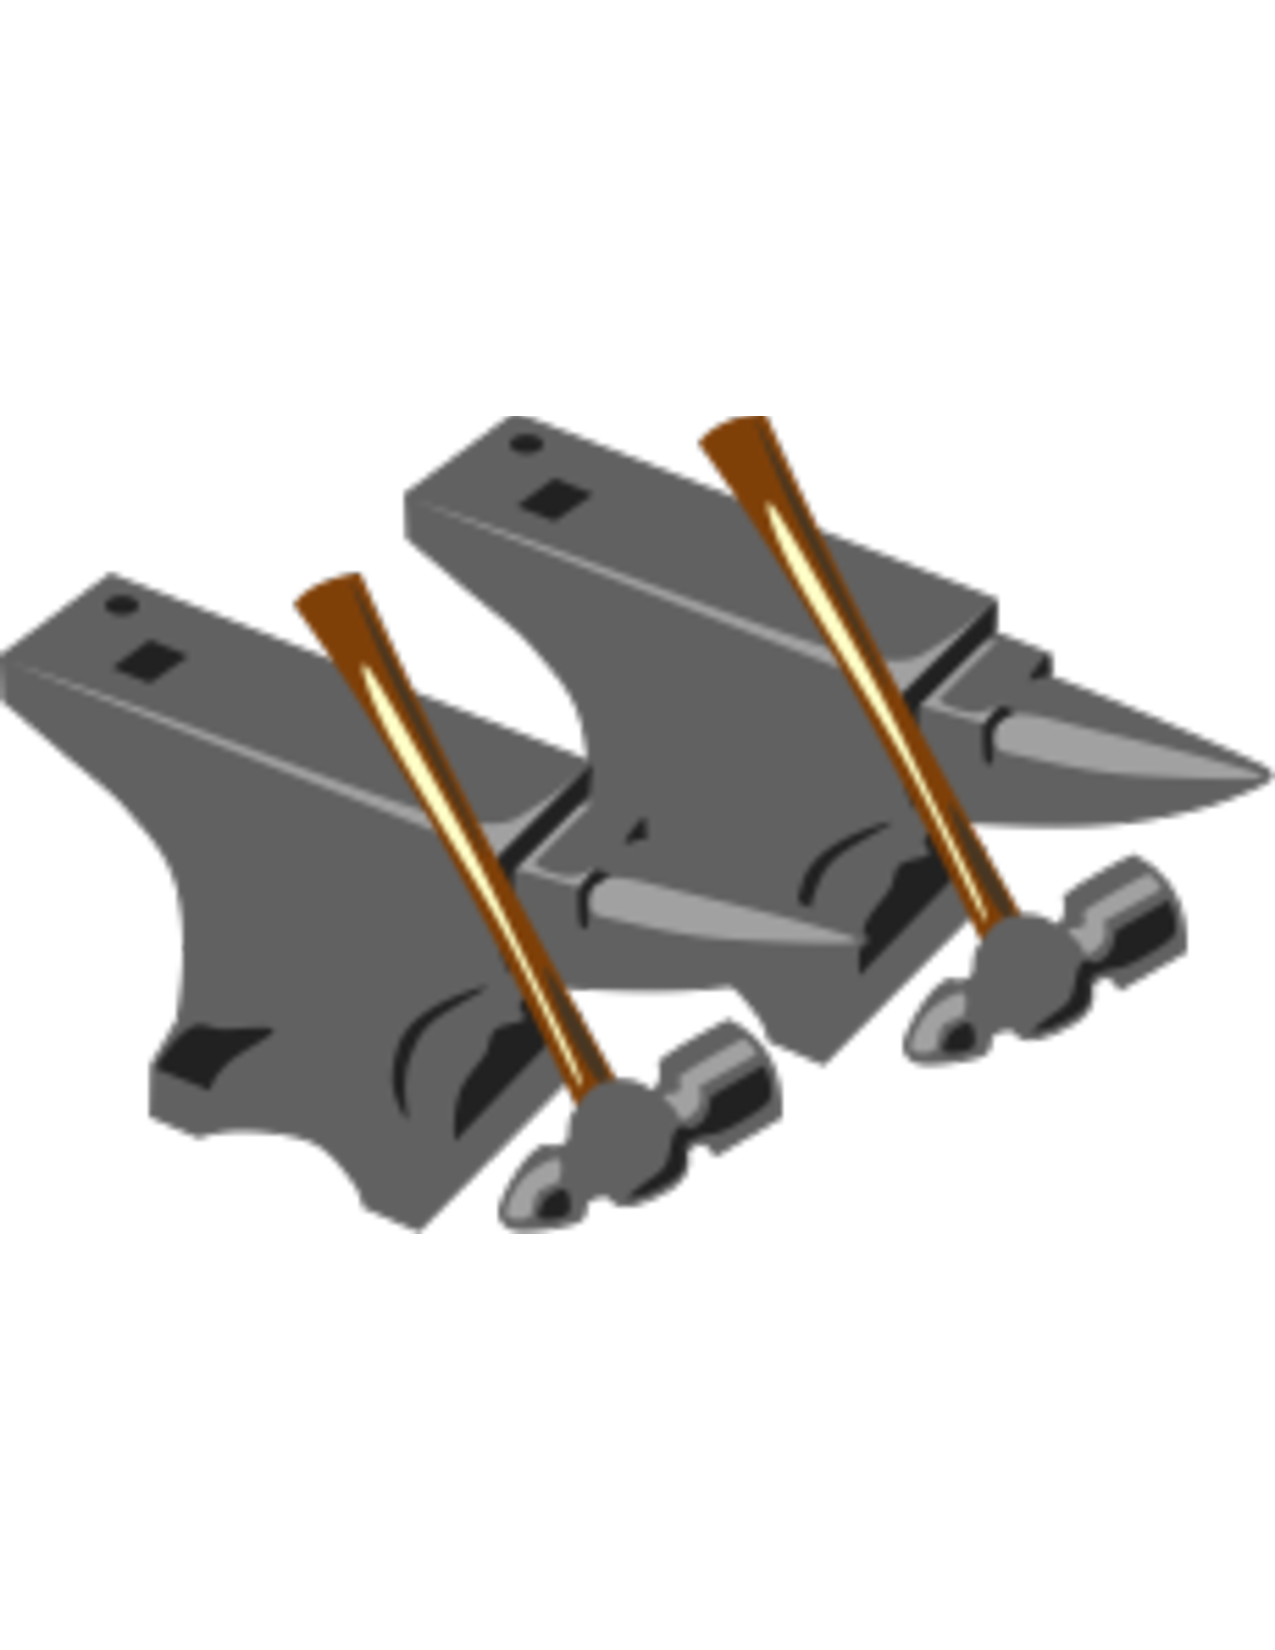
\includegraphics[width=0.4\columnwidth]{logo}
\end{figure}
\newpage
\tableofcontents
%\listoffigures


% \input{title}

\newpage
\section{Introduction}
\subsection{What is RapidSmith 2?}
The original BYU RapidSmith project began in 2010. Its goal was to develop
a set of tools and APIs which would provide academics with an
easy-to-use platform to implement experimental CAD ideas and algorithms on
modern Xilinx FPGAs. It integrated with Xilinx's old design suite, ISE.
RapidSmith 2 (abbreviated RS2 hereafter) represents a major addition to
RapidSmith. Specifically, Vivado designs are now supported. Using RS2 you can
write custom CAD tools which will:
\begin{itemize}
  \item Export designs from Vivado
  \item Perform analyses on those designs
  \item Make modifications to those designs
  \item Import those designs back into Vivado for further processing or
  bitstream generation
\end{itemize}
Futhermore, you need not start with a Vivado design --- 
you can create a new design from scratch in RS2 and then import it into Vivado
if desired.

The other new major capability of RS2 is that it changes RapidSmith's design
representation. Instead of using XDL's view of a design with Instances and
Sites, RS2 uses Vivado's representation of design with Cells and BELs. This
is a significant change as it exposes the actual design and device in a way
that RapidSmith never did, opening up new CAD research opportunities which were
difficult to perform using Rapidsmith.
       
\subsection{Who Should Use RS2?}
RS2 is aimed at anyone desiring to do FPGA CAD research on real Xilinx devices
available in Vivado. As such, users of RS2 should have some understanding of
Xilinx FPGA architecture, the Vivado design suite, and the Tcl programming
language. However, one goal of this documentation is to provide sufficient
background and detail to help bring developers up to speed on the needed
topics. RS2 is by no means a Xilinx Vivado replacement. It cannot be used
without a valid and current license to a Vivado installation (RS2
cannot generate bitstreams for example).

\subsection{Why RS2?}
The Xilinx-provided Tcl interface into Vivado is a great addition to the tool
suite. It can be used to do a variety of useful things including scripting
design flows, querying device and design data structures, and  modifying placed
and routed designs. In theory, the Tcl interface provides all of the
functionality needed in order to create any type of CAD tool as a plugin to the
normal Vivado tool flow. However, there are a few issues in TCL that motivate
the use of external CAD tool frameworks such as RS2. These include:
\begin{itemize}
  \item Tcl, being an interpreted language, is slow. It is far too slow to
  implement complex algorithms such as PathFinder. Compiled and
  managed runtime languages are a better option in terms of performance.
  \item Tcl is hard to program in. TCL is not an object oriented language, and
  so writing complex algorithms are difficult since Object-Oriented language
  constructs do not exist. That being said, TCL is great for writing automation
  scripts.
  \item There are some memory issues in Vivado's Tcl interface. In our
  experience, long-running scripts eventually cause the system to run out of
  memory even if they are not doing anything interesting.
  \item Vivado's TCL interface does not offer a complete device representation
  (determined by Brad White's MS work). Most notably, a user cannot gain
  access to sub-site wire objects through the Tcl interface. This limits the CAD
  tools that can be created in Tcl, but this additional information can be added
  to external tools with some manual work.
\end{itemize}

\noindent
In short, the ability to export designs out of Vivado, manipulate them with more
powerful languages such as Java, and then import the design back into Vivado
is a very useful capability.

RS2 (in conjunction with Tincr which is described in \autoref{sec:tincr})
abstracts this process into a few easy-to-use function calls. Generating FPGA
part information, importing and exporting \pgm{all aspects} of a design, and
dealing with other fairly arcane details is made mostly transparent to the
user. RS2 and Tincr provide a nice API into equivalent Vivado device and design
data structures. All of this enables researchers to have more time to focus on what matters
most: the research of new ideas and algorithms.

\subsection{Which Xilinx Parts does RS2 Support?}
As of the writing of this document, Artix 7 has been tested the most and is
currently supported in all forms and applications.  In addition, an Ultrascale
device file was created and demonstrated as a part of Brad White's MS work to
show that it is possible. At some point, Ultrascale should be fully supported.
\footnote{An XDL-based import/export capability has also been created and used
with Virtex 6 devices as a part of Travis Haroldsen's PhD work but that path is
not being released, documented, or supported.}

As will be seen later, to generate additional device files for additional parts
within a supported family is relatively straightforward and can be done by any
user.  New families can also be supported but this
requires a bit more work.  As time goes on the process will become simpler ---
that is one of the goals for RS2 moving forward.

\subsection{How is RS2 Different than VPR and VTR?}
VPR (Versatile Place and Route) has been an FPGA research tool for several years
and has led to many publications on new FPGA CAD research. It has been a
significant contribution to the FPGA research community and has grown to be a
complete FPGA CAD flow for research-based FPGAs. The main difference between
RapidSmith and VPR is that the RapidSmith tools can target commercial Xilinx
FPGAs, providing the ability to exit and re-enter the standard Xilinx flow at
any point.  All features of commercial FPGAs which are accessible via XDL and
Vivado's Tcl interface are available in RapidSmith and RS2. VPR is currently
limited to FPGA features which can be described using VPR's architectural
description facilities.

\subsection{Why Java?}
RS2 is written in Java. We have found Java to be an excellent rapid prototyping
platform for FPGA CAD tools.  Java libraries are rich with useful data
structures, and garbage collection eliminates the need to clean up objects in
memory. This helps reduce the time spent debugging, leaving more
time for researchers to focus on the real research at hand.  Our experience over
the past decade is that for student research projects, Java has greatly improved
student productivity and led to far more stable CAD tools.

\pagebreak
\section{Vivado, RS2, and Tincr}
\subsection{RapidSmith vs. RS2}
\subsubsection{What Was The Original RapidSmith?}
The original RapidSmith was written by Christopher Lavin as a part of his PhD
work at BYU.  It was based on the Xilinx Design Language (XDL) which provides a
human-readable file format equivalent to the Xilinx proprietary Netlist Circuit
Description (NCD) of ISE.  With RapidSmith, researchers were able to import
XDL/NCD, manipulate, place, route and export designs among a variety of design
transformations.  The RapidSmith project made an excellent test bed to try out
new ideas and algorithms for FPGA CAD research because code could quickly be
written to take advantage of the APIs available.

RapidSmith also contained packages which could parse/export bitstreams (at the
packet level) and represent the frames and configuration blocks in the provided
data structures.  In this regard, RapidSmith did not include any proprietary
information about Xilinx FPGAs that is not publicly available.

RapidSmith continues to be functional and is still available at the
SourceForge.net website.  There, you will find documentation, installation
instructions, the RapidSmith code base, and a collection of demo programs based
on it.

\subsubsection{What is RS2?}
With the announced end of ISE (with the Virtex7 family of parts being the last
family to be supported by ISE), there was no path forward to newer parts using
RapidSmith.  This is because XDL is not available with Vivado. With
Vivado, however, Xilinx has provided an extensive Tcl scripting capability which 
initially looked as if it could provide a similar capability to that provided by
XDL in terms of accessing both Vivado's design and device data and in terms of
creating and modifying Vivado designs.  However, as described above, Vivado's
Tcl is limited by speed and memory challenges.
The development of RS2 consisted of three parts.

\subsubsection{Tincr: Integrating Custom CAD Tool Frameworks with the Xilinx 
Vivado Design Suite} \label{sec:tincr}

In the first part, the Vivado Tcl capability was investigated to ensure that,
indeed, it did provide the needed ability to access design and device data and
export that to external tools such as RapidSmith.  This resulted in the Tincr
project, led by Brad White as a part of his MS work at BYU, with Thomas
Townsend making additions as a part of his research.

Tincr is a Tcl-based library of routines which (a) provide a variety of
functions to simply make working with Vivado via Tcl easier, (b) provide a way
to export all the data associated with a Vivado design into what is called a
Tincr Checkpoint (TCP), (c) provide a way to reimport Tincr Checkpoints back
into Vivado, and (d) access device data from Vivado and output that data in the
form of XDLRC files (these are the files which XDL used to describe devices and
are necessary for RapidSmith and RS2 to understand the structure of and the
resources available for use in a given Xilinx part).  Tincr is available at 
\href{https://github.com/byuccl/tincr}{\color{blue}https://github.com/byuccl/tincr}.
Tincr is described in two publications:

\begin{quotation}B. White and B. Nelson, "Tincr — A custom CAD tool framework
for Vivado," 2014 International Conference on ReConFigurable Computing and FPGAs (ReConFig14),
Cancun, 2014, pp. 1-6, DOI: 10.1109/ReConFig.2014.7032560

White, Brad S., "Tincr: Integrating Custom CAD Tool Frameworks with
the Xilinx Vivado Design Suite" (2014), BYU Scholars Archive, Paper 4338. 
\\URL:http://scholarsarchive.byu.edu/etd/4338
\end{quotation}

\subsubsection{RS2: A Framework for BEL-Level CAD Exploration on Xilinx FPGAs}
The second part of the development of RS2 was to add a new layer of design
representation to RapidSmith which more closely matches that of Vivado.  This
was done as a part of his PhD work by Travis Haroldsen at BYU.  As of this
writing, one paper on RS2 has appeared:

\begin{quotation}Travis Haroldsen, Brent Nelson, and Brad Hutchings, “RapidSmith
2:
A Framework for BEL-Level CAD Exploration on Xilinx FPGAs�, Proceedings of the
2015 ACM/SIGDA International Symposium on Field-Programmable Gate Arrays,
February 2015, Monterey CA, pp. 66-69, DOI: 10.1145/2684746.2689085.
\end{quotation}

\subsubsection{Vivado and RS2 Integration}
The third part of the development of RS2 was to create the ability to export
designs from Vivado and into RS2 and, correspondingly, to import RS2 data back
into Vivado.  This was completed during 2016, largely by Thomas Townsend
as an MS student at Brigham Young University.  The initial
public release of RS2 was made in January 2017 once that piece was in place.

\subsubsection{What is All This About XDL and XDLRC and How Does RS2 Fit Into
That?} 
The Xilinx ISE tools had the capability to export XDL and XDLRC files which
RapidSmith used: 
\begin{itemize}
  \item An XDLRC file was a complete description of a given Xilinx FPGA,
  describing every tile, every switchbox, every wire segment, and every PIP in
  the part.  RapidSmith was able to process this information and create a device
  representation for use in support of CAD tools such as placers and routers.
  \item An XDL file was a textual representation of an NCD file (a user design).
  It described the user design as a collection of \cls{Instances} and \cls{Nets}. Instances
  correspond to things like {SLICEs}, {BRAMs}, {DSP48s}, and {IOBs}.  Instances could be
  placed onto \cls{Sites}. Additionally, Nets in XDL consisted of a list of
  \cls{Pins} (their logical connections) and an optional list of \cls{PIPs} (their physical
  routing connections).
\end{itemize}
In Vivado, however, designs are described as a collection of \cls{Cells} where a Cell
corresponds to things like LUTs, flip flops, etc.  A Cell may be placed
onto a \cls{BEL} object such as an ALUT or a BFF.  RS2 contains a new layer of
hierarchy in its design and device descriptions where Cells and BELs are first-class objects and
design manipulation is all done at the Cell/BEL level.

Also, Vivado Nets are described using directed routing strings rather than lists
of PIPs.  RS2 also contains a set of new classes to enable the representation
and manipulation of Nets in a format compatible with these routing strings.

Thus, using RS2, design manipulation is now done at the level of Cells and BELs
and importing/exporting designs to/from Vivado is now fully supported.

\subsection{RS2 Usage Model and Structure}
The usage model for RS2 is shown in \autoref{fig:UsageModels}.  As can be
seen, a design can be exported from Vivado at multiple different points in the
Vivado design flow.  In each case, Tincr is used to export a Tincr Checkpoint
which can then be imported into RS2.  At those same points in the design flow,
RS2 can export a Tincr Checkpoint which can then be imported back into Vivado. 
Thus, a complete solution involves Vivado, Tincr, and RS2.

\begin{figure}[htb]
\centering
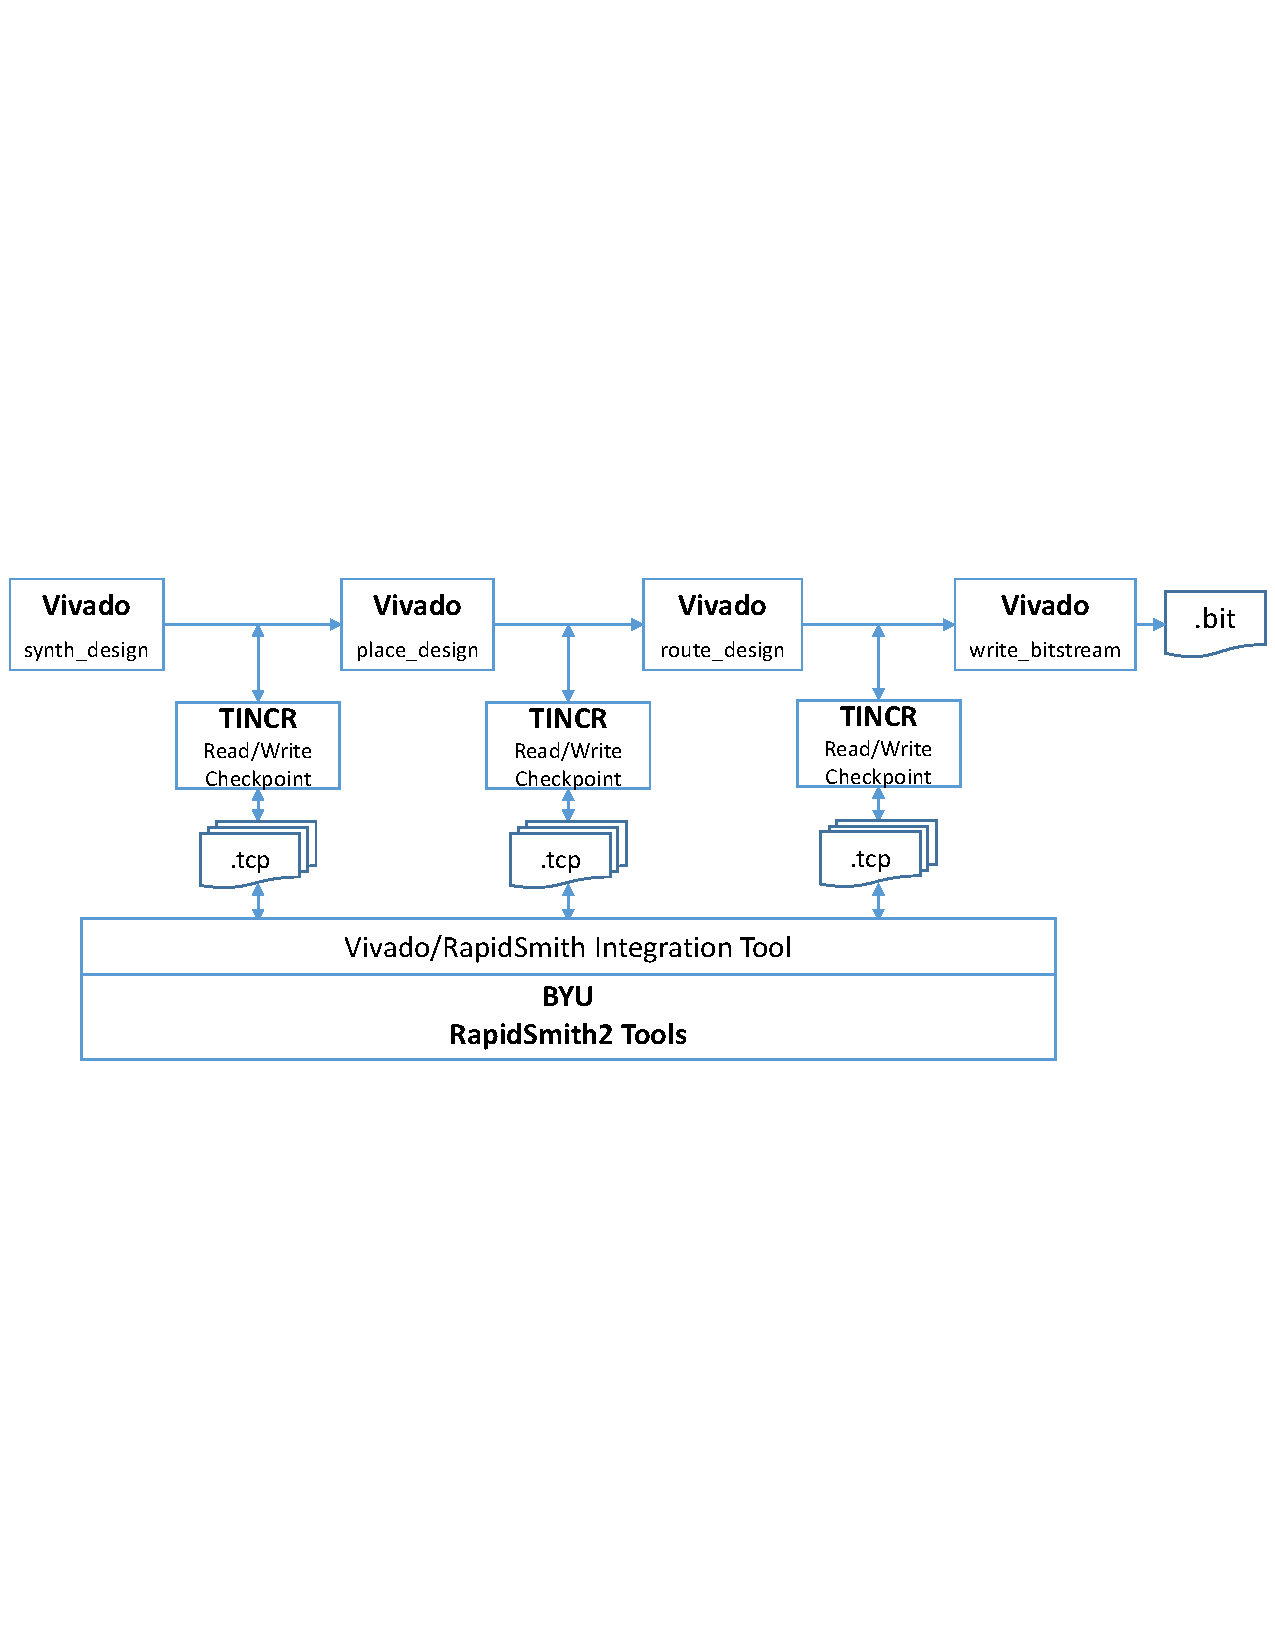
\includegraphics[width=\columnwidth]{UsageModels}
\caption{Vivado and RS2 Usage Model}
\label{fig:UsageModels}
\end{figure} 

\pagebreak
\section{Getting Started}

\subsection{Installation}

RS2 is available on Github at:
{\color{blue}{\url{https://github.com/byuccl/RapidSmith2}}}.
You can either build RS2 into .class and .jar files for use in any Java
environment, or configure RS2 to work in an IDE (recommended).

\subsubsection{Requirements for Installation and Use}
\begin{itemize}
  \item Windows, Linux or Mac OS X all will work (see additional notes below for
  Mac OS X)
  \item Vivado 2016.2. Later versions of Vivado may work, have not been tested
  yet. Earlier versions will not work.
  \item JDK 1.8 or later
  \item Tincr 
\end{itemize}

Tincr is a companion project
({\color{blue}{\url{https://github.com/byuccl/tincr}}}) which is used for
importing/exporting designs between Vivado and RS2.  For getting started (running the example programs on the provided sample designs) you will not need it installed.
Later, as you  actually start processing your own Vivado designs you will need
to obtain and install it. There are additional dependencies beyond these
required for installation, but they are either provided in the distribution
itself or are automatically retrieved for you as a part of the installation process. 
Examples of these additional dependencies include QT Jambi and the BYU Edif
Tools.
 
\subsubsection{Steps for Installation}

\begin{enumerate}
  \item Clone the RS2 repository at
  {\color{blue}{\url{https://github.com/byuccl/RapidSmith2}}}. If you are not
  familiar with GitHub, you will need to install Git on your computer, and run the
  following command in an open terminal: 
  \begin{code}
  git clone https://github.com/byuccl/RapidSmith2
  \end{code} 
  \noindent This will copy the RS2 repository into a local directory.
  \item Create a new environment variable called RAPIDSMITH\_PATH, and point it
  to your local repository of RS2 that you setup in step (1). This is needed so
  RS2 can find required device files and other items at runtime.
  \item Build the  RS2 project. RS2 is managed using a gradle build system.
  To build the project, navigate to your local repository of RS2 and execute one
  of the following scripts in a terminal:
  \begin{code}
	gradlew build (unix)
	gradlew.bat build (windows)
  \end{code}
  The build process could take a few minutes.
  \item At this point, you have two choices: set up RS2 for use in an IDE, or
  run RS2 from the command line. Both choices are detailed below.
  \paragraph{Running from an IDE} The gradle scripts in RS2 currently support
  setup for both Eclipse and IDEA Java IDEs. This section will detail how to
  setup the Eclipse environment, but similar steps can be taken for IDEA. If
  using Eclipse, it is best to use version Eclipse Neon or later. To create a
  new eclipse project, execute one of the following in a terminal:
  \begin{code}
	gradlew antlr eclipse (unix)       
	gradlew.bat antlr eclipse (windows)
  \end{code}
  Executing these will create an Eclipse \fil{.project} file. After the project
  file has been created, you can import the project into Eclipse by opening
  Eclipse and selecting:
  \begin{code}
	File->Open Projects From File System 
  \end{code}
  and pointing it to your RapidSmith2 local repository. All Java source files
  will be found under \dir{src/main/java}. \pgm{NOTE:} Your RS2 git repository
  should not be put inside your eclipse workspace. It is better to put it
  elsewhere, and then import it into your workspace.
  \paragraph{Building on the Command Line} After step (3) in the installation
  process, gradlew produces everything that you will need to run RS2 from the
  command line. The following directories are created: 
  \begin{itemize}
    \item \fil{build/classes/main}: This folder contains the RS2 class file
    directory tree.
    \item \fil{build/libs}: This folder contains a Jar file of the RS2 class
    files.
    \item \fil{build/distributions}: This folder has both .zip and .tar files
    with contains all Jars needed to run RS2 from the command line. This
    includes a full jar of the RS2 build alond with copies of dependency Jars
    (such as QT-Jambi).
  \end{itemize} 
  After adding the appropriate .class files or Jars to your \texttt{CLASSPATH},
  you should be able to run RS2 tools from the command line. If you make any
  changes to the RS2 code, you will have to rebuild before running the program
  again (Step 3). \pgm{CAUTION:} An obvious thing to try is to mix and match
  developing in Eclipse but then running the resulting apps from the command
  line. Just be aware that Eclipse puts its compiled .class files in very
  different places than where the gradle build process puts its .class and
  .jar files. Make sure you understand that before you try to combine these two
  build/execution methods. Our suggested approach is to choose one or the
  other, but not both.
\end{enumerate}

\subsubsection{Additional Notes for Mac OS X Installation}

The instructions above require you to set the \env{RAPIDSMITH\_PATH}
environment variable.  If running from the command line, the environment
variables can be added to your \fil{.bash\_profile} file as in any other
UNIX-like system.  However, if using an IDE such as Eclipse you either need to
define the environment variable for every Run Configuration you create, or you
need to add the \env{RAPIDSMITH\_PATH} definition system-wide in OS X. This can
be done, but how to do so differs based on what OS X version you are running
(and seems to have changed a number of times over the years). Search the web for
instructions for how to do so if you desire. \pgm{Hint}: you will likely have
to edit some \fil{.plist} files.

\subsubsection{Running RS2 Programs}
Some points to keep in mind while configuring and running RS2 programs:
\begin{itemize}
  \item The RS2 code base contains a number of assertions which may be helpful  
  as you are developing code.  These are not enabled by default in Java.  To
  enable them, add \opt{-ea} as a VM argument.  This is highly recommended.
  \item If you are running on a Mac, when running RS2 programs that use Qt  (any
  of the built-in programs like \pgm{DeviceBrowser}) that are GUI-based, you
  will need to supply an extra JVM switch, \opt{-XstartOnFirstThread}.
  \item A common error when running RS2 programs is failing to have your
  \env{RAPIDSMITH\_PATH} defined.  If this is the case when you try to execute a
  program, an \texttt{EnvironmentException} will be thrown telling you that you
  forgot to set the variable.
  \item If you are running on Windows, only a 32-bit QT Jar file is included in
  the RS2 repository. This means that you will need to set your JRE to a 32-bit
  version when running the GUI programs. We are working on updating QT to the
  latest version, so this will no longer be an issue.
  \item For Linux command line usage, the \env{CLASSPATH} environment variable
  must point to both the full (uncompressed) RS2 jar in the \dir{build/distributions}
  folder as well as all the jar files in the \dir{/lib} subdirectory. An example
  \env{CLASSPATH} could look like this:
  \vspace{-0.15in}  \begin{code}
  Â  Â  Â RAPIDSMITH2-SNAPSHOT/*:RAPIDSMITH2-SNAPSHOT/lib/*
  \end{code}
\end{itemize}

\subsubsection{Testing Your Installation}
\noindent At this point you can test your installation by executing the java
\pgm{DeviceBrowser} program: 
\vspace{-0.15in}  \begin{code}
java edu.byu.ece.rapidSmith.device.browser.DeviceBrowser
\end{code}    

\noindent This can be done either from within Eclipse or from the command line,
depending on how you are running RS2 (if running under OS X be sure to provide the
\opt{-XstartOnFirstThread JVM argument}. If all goes well you should see a
graphical representation showing the details of a physical FPGA device as shown
in \autoref{fig:deviceBrowser}.  You may initially be zoomed far in and might
want to zoom out to see the entire chip layout.

\begin{figure}[H]
\centering
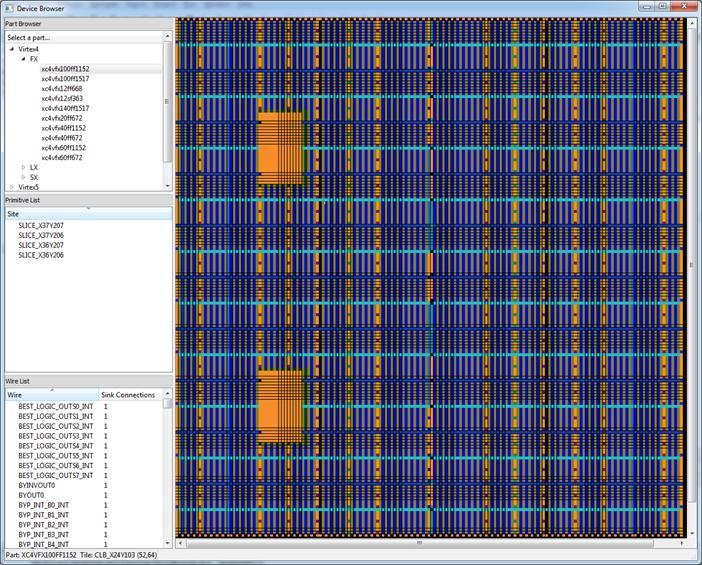
\includegraphics[width=0.8\columnwidth]{deviceBrowser}
\caption{\pgm{DeviceBrowser} Sample Display}
\label{fig:deviceBrowser}
\end{figure}

\subsection{Device Files For Use With RS2}
Device files for one part (the {\em xc7a100tcsg324}) are included in the
distribution so you can immediately start working with RS2 (initially, it
will be the only device available when you run the \pgm{DeviceBrowser} program
above).  The device files for this part can be found in the
\dir{\${RAPIDSMITH\_PATH}/devices/artix7} directory. If you desire to work with
additional parts, follow the instructions found in the file
\fil{\$RAPIDSMITH\_PATH/\-doc/Installing\-NewDevices.txt}.

\clearpage
\section{Devices in RS2}

\subsection{Xilinx FPGA Architecture Overview} \label{fpgaArch}
This section is intended to give a brief introduction to Xilinx FPGA
architecture and terminology. The terminology introduced here is consistent
with the terminolgy used in the Vivado Design Suite. If you are already familiar
with Xilinx FPGA devices, then you can skip to \autoref{devicesRS2}. 
As you read through this section, it may be helpful to open a sample device in Vivado's
Device Browser. To do this, open a new command prompt and run Vivado in Tcl mode
(``vivado -mode tcl''). Then, run the following commands in the Vivado prompt:

\begin{verbatim}
Vivado% link_design -part xc7a100tcsg324-3 -quiet
Vivado% start_gui
\end{verbatim}

\noindent
After these commands are run, a GUI view should pop up showing the components
of an Artix7 FPGA part. Use this to explore the Xilinx device architecture if
needed.

\subsubsection{Tiles}
Conceptually, a Xilinx FPGA can be thought of as a two dimensional
array of \cls{Tile}s. A \cls{Tile} is a template section within a FPGA that
performs a specific function (say, implementing logic equations). Templates are
then duplicated across the device (all copies are identical) and different
\cls{Tile} types are wired together. As an example, \autoref{fig:tileExample}
displays three types of template \cls{Tile}s in an Artix7 part.

\begin{figure}[H]
 \centering
 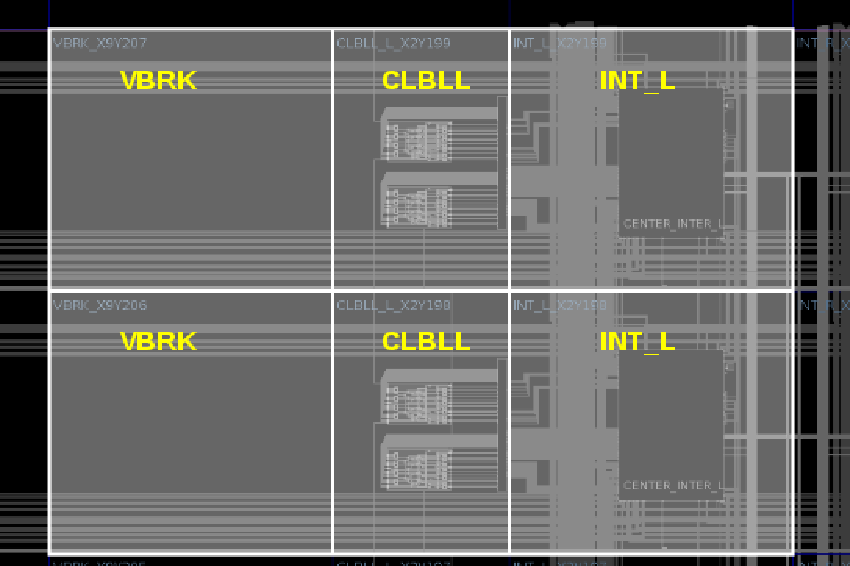
\includegraphics[width=0.7\columnwidth]{tiles}
 \caption{Highlighted example \cls{Tile}s in an Artix7 FPGA.}
 \label{fig:tileExample}
\end{figure}

\noindent
The two \pgm{VBRK} \cls{Tile}s on the left are used for intermediate wiring.
The two \pgm{INT\_L} \cls{Tile}s on the right are switchbox \cls{Tile}s.
These are reconfigurable routing \cls{Tile}s that allow a single wire to go
multiple different locations within the FPGA. The two \pgm{CLBLL} \cls{Tile}s
in the middle are used to implement combinational and sequential digital logic.
They are the basic building blocks of Xilinx FPGAs. Other \cls{Tile} types
include DSP, BRAM, and IOB.
 
\subsubsection{Primitive Sites}

\begin{figure}[b!]
\centering
   \begin{subfigure}[b!]{0.65\textwidth}
   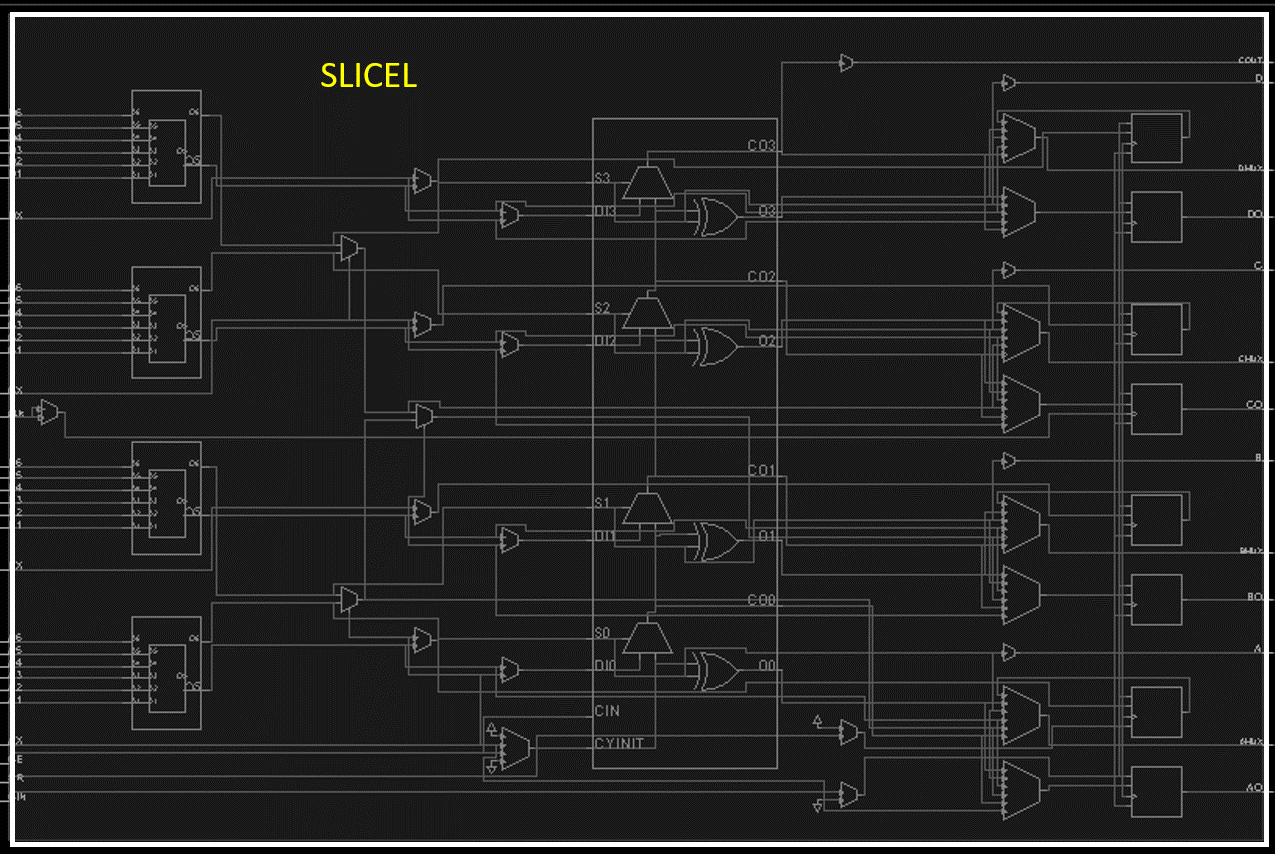
\includegraphics[width=1\linewidth]{site}
   \caption{}
   \label{fig:site1} 
\end{subfigure}

\begin{subfigure}[b!]{0.65\textwidth}
   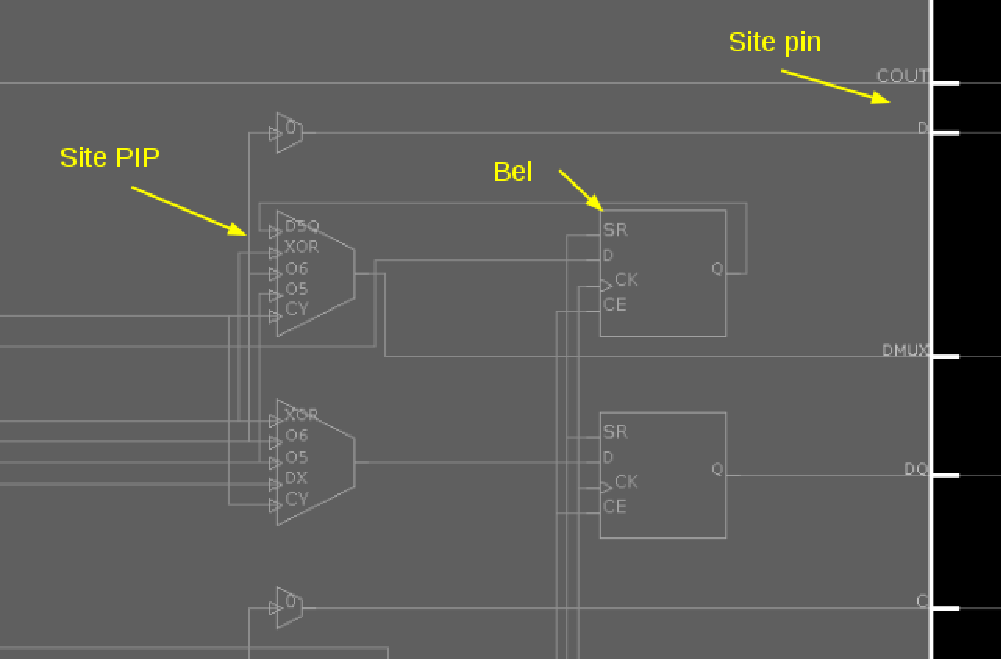
\includegraphics[width=1\linewidth]{subsite}
   \caption{}
   \label{fig:site2}
\end{subfigure}

\caption{(a) A highlighted example of a SLICEL \cls{Site} in a CLBLL \cls{Tile}
of an Artix7 FPGA. (b) The basic components of a \cls{Site} in a
Xilinx FPGA.}
\label{fig:site}
\end{figure}

Each \cls{Tile} can contain one or more \cls{Primitive Site}s (often shortened
to \cls{Site}). As \autoref{fig:tileExample} shows, CLBLL \cls{Tile}s
have two \cls{Site}s, INT\_L \cls{Tile}s have one \cls{Site}, and VBRK \cls{Tile}s
have none. A \cls{Site} is the part within a \cls{Tile} that actually performs
its ``useful'' function. The remainder of the \cls{Tile} is used to wire signals
to/from its \cls{Site}s. \autoref{fig:site} shows a SLICEL, one of the
\cls{Site}s within a CLBLL \cls{Tile}. As the figure shows, there are three main
components to \cls{Site}s in Xilinx FPGAs:

\begin{itemize}
  \item \cls{Site} \cls{PIP}s: Reconfigurable routing PIPS used for intrasite
  routing (also called routing muxes). In Vivado, \cls{Site} \cls{PIP}s are usually configured
  automatically as cells in a design are being placed (based on cell properties
  and placement location).
  \item \cls{BEL}s: \pgm{B}asic \pgm{EL}ements are hardware components within
  the \cls{Site} for implementing digital logic. For example, LUT \cls{BEL}s within a SLICEL
  are used to implement logic equations, and Flip Flop \cls{BEL}s are used
  as storage. In a synthesized netlist, design elements are mapped to physical
  \cls{BEL}s during implementation.
  \item \cls{Site Pin}s: \cls{Site} input and output. These pins are connected
  to \cls{Wire}s of the parent \cls{Tile} and typically drive general
  fabric.
\end{itemize}

\subsubsection{Wires and PIPs} \label{wireSection}
 
FPGA components are connected together using metal \cls{Wire}s (called
\cls{Node}s in Vivado). In order to make the FPGA reconfigurable,
\cls{Wire}s are connected together through Programmable Interconnect Points
(\cls{PIP}s). Individual \cls{PIP}s can be enabled or disabled as a design is
being routed, and a string of enabled \cls{PIP}s uniquely identify the
used \cls{Wire}s of a physical route. \cls{PIP}s are most commonly
found in Switchbox \cls{Tile}s, and enable a single wire to be routed to many
different locations in the FPGA. \autoref{fig:switchboxPIP} shows an
example of a switchbox.

\begin{figure}[H]
	\centering
	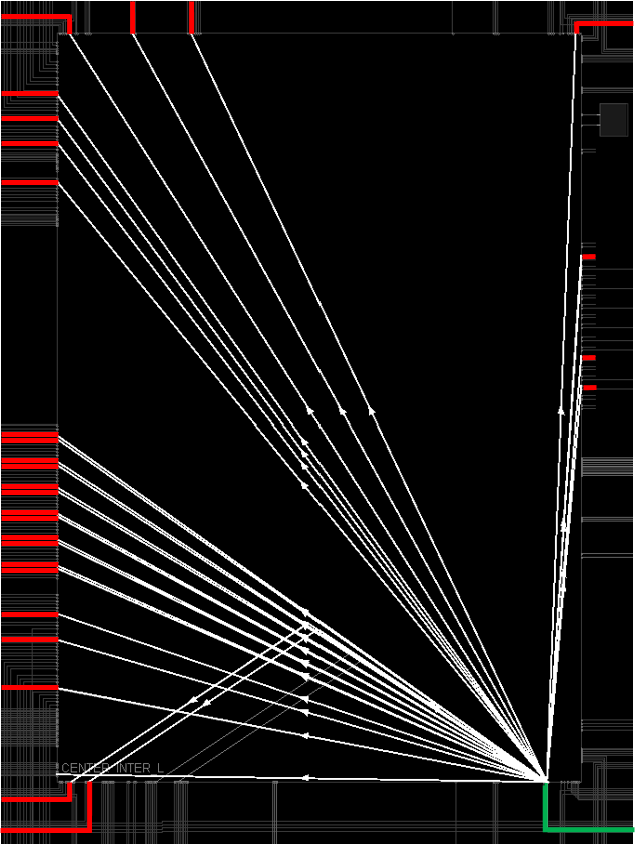
\includegraphics[width=0.45\columnwidth]{pipExample}
	\caption{An example of PIP wire connections in a device. The green wire
	represents the source wire, and the red wires represent all possible sink
	wires in the Switchbox. The highlighed white sections of the figure are PIP
	connections.}
	\label{fig:switchboxPIP}
\end{figure} 
 
\subsection{Device Data Structures} \label{devicesRS2}
In the original RapidSmith, the \cls{Device} architecture stopped at the
\cls{Site} level. A \cls{Site} was considered a black box who could be
configured using string attributes, but the actual components were unknown.
RapidSmith 2 extends the \cls{Device} architecture to include all components
\pgm{within} a \cls{Site} as well. \autoref{fig:deviceDataStructures}
shows the new data structure hierarchy, which can be found in the {\em
edu.byu.ece.rapidSmith.device} package.

\begin{figure}[H]
	\centering
	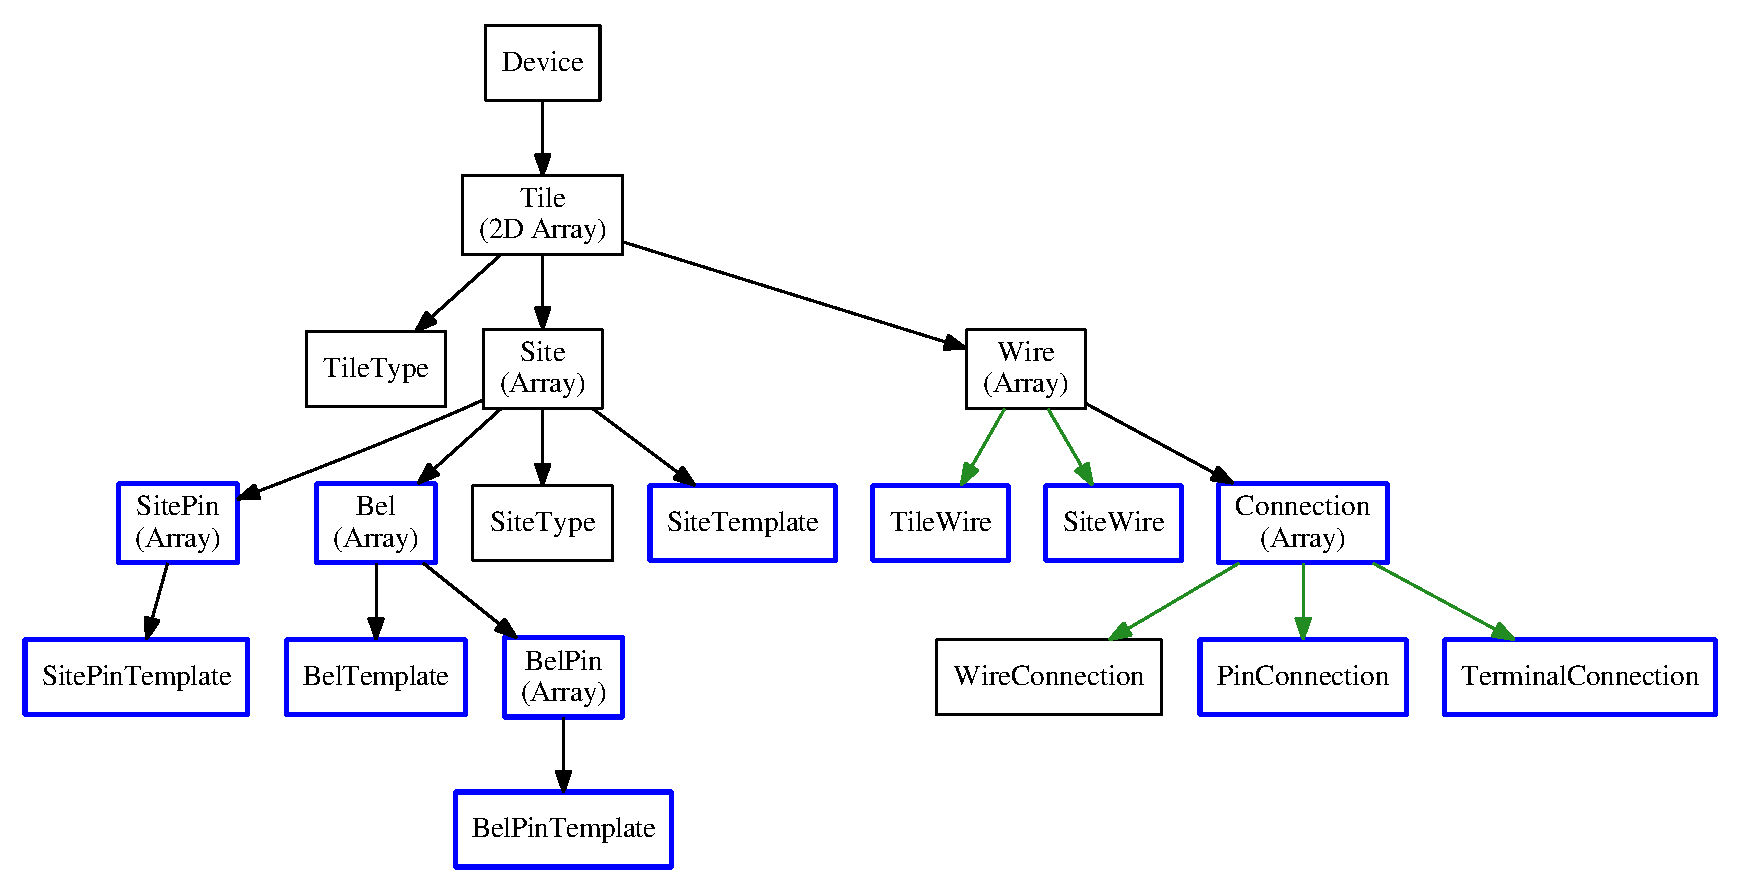
\includegraphics[width=1\columnwidth]{deviceDS.eps}
	\caption{RapidSmith2 \cls{Device} data structure tree. Green arrows represent
	inheritance, and black arrows represent association. Classes and Interfaces
	bolded in blue are new to RapidSmith 2.}
	\label{fig:deviceDataStructures}
\end{figure}

\noindent
The classes and interfaces within {\em edu.byu.ece.rapidSmith.device} are named
to reflect the terminology used by Xilinx. Many classes that exist in Vivado's
Tcl interface have a direct map to a class in RapidSmith (such as a \cls{Tile}).
Because of this, most RapidSmith data structures represent a straightforward
part of a Xilinx FPGA, The reader is referred to the documentation in the
source code to learn more about each data structure. Also, The
\pgm{DeviceBrowser} and \pgm{DeviceAnalyzer} programs described in 
\autoref{examples} illustrate how to load and browse a device down to the
\cls{Tile} and \cls{Site} levels.

\subsubsection{Templates}
As \autoref{fig:deviceDataStructures} shows, there are several template
classes in RapidSmith. Template classes are used to specify the configuration of
certain structures only once, and then reuse the configuration across
identical objects. The usefulness of templates is best shown with an example. In
an Artix-7 {\em xc7a100tcsg324} part, there are 11,100 \cls{Site}s of type
SLICEL. Each of these SLICELs have 215 \cls{BEL}s, \cls{Site} \cls{Pin}s, and
\cls{Site} \cls{PIP}s combined. In order to save memory, RapidSmith
lazily creates these objects only when a SLICEL \cls{Site} is being used. The
alternative would be to create each of the objects when a device is loaded.
Template classes should \pgm{NOT} be used by the normal user. When creating
algorithms using RapidSmith's API, use the non-template version of classes.

\subsubsection{WireEnumerator} \label{wireEnum}
Wires with the same name can occur several times throughout a Xilinx FPGA
device. For example, the wire ``CLBLL\-\_L\_C2'' exists in every \cls{Tile} of
type ``CLBLL\_L''. In order to make the device files small, each uniquely named \cls{Wire}
is assigned an integer enumeration. This avoids moving strings around in
memory which would be costly in terms of both space and comparison times.
RapidSmith manages all uniquely named wires in an FPGA family with a
\cls{WireEnumerator}. The \cls{WireEnumerator} class has methods that convert to
and from the wire name and enumeration of a \cls{Wire}, and also stores other
\cls{Wire} information such as direction and type. In previous versions of
RapidSmith, the user had to use the \cls{WireEnumerator} extensively while
building CAD tools. RapidSmith 2 has changed this, largely abstracting the
\cls{WireEnumerator} away in favor of more convenient methods in all classes and
interfaces that deal with \cls{Wire}s. For example, the name or enumeration of a
\cls{Wire} can now be obtained with the function calls {\em Wire.getWireName()}
and {\em Wire.getWireEnum()} respectively. A handle to the
\cls{WireEnumerator} still exists in the \cls{Device} class for those who
want to use it, but this is not recommended. 

\subsubsection{TileWire and SiteWire} \label{wires}
\cls{Wire}s in RapidSmith are uniquely identified not only by their name
(or enumeration), but also by the \cls{Tile} or \cls{Site} in which they exist.
RapidSmith 2 introduces the \cls{TileWire} and \cls{SiteWire} classes to
encapsulate this information for the user. Many functions in RapidSmith now
return a \cls{TileWire} or \cls{SiteWire} (wrapped in a generic \cls{Wire}
object) to the user instead of an integer wire enumeration.

\subsubsection{Wire and Connection Interfaces}
As \autoref{fig:deviceDataStructures} shows, there are two classes that
inherit the \cls{Wire} interface (described in \autoref{wires}) and
three classes that inherit the \cls{Connection} interface (described in 
\autoref{otherConns}). In general, most methods in RapidSmith return the
generic interface instead of the subclasses. When creating CAD tools in
RapidSmith, it is suggested that the user use these interfaces. Several of the
examples referenced in \autoref{examples} demonstrate the use of these
interfaces.

\subsection{Device Files}
The \cls{Device} data structures in RapidSmith are created from XDLRC files.
For older Xilinx parts (series 7 and below), these files can be created
in ISE with the {\em xdl} command. For newer parts (ultrascale and
above), XDLRC files can be created in Vivado using the TINCR command
{\em tincr\-::write\_xdlrc}. Because XDLRC files can
grow to be hundreds of Gigabytes in size, RapidSmith compresses them into much
smaller device files (usually in the tens of Megabytes) and stores those
instead. This section gives a brief overview of the syntax of XDLRC files, and
how to install new device files in RapidSmith from both ISE and Vivado.

\subsubsection{Basic Syntax of XDLRC files}
In general, users of RapidSmith do not need to understand the syntax of XDLRC
files to create CAD tools in RapidSmith. The syntax is introduced here for those
who are interested, and for those who want to modify the XDLRC parser
in some way. If these don't apply to you, then go ahead and skip this section.
XDLRC files are textual descriptions of Xilinx FPGA devices and can be very
verbose (which is why they get so large). This section highlights the main parts
of an XDLRC file with accompanying images. As you will see, much of the
terminology is the same as \autoref{fpgaArch}.

\bigbreak \noindent
\begin{large}
\pgm{Tiles}
\end{large}

\begin{figure}[H]
	\centering
	
\includegraphics[width=1\columnwidth]{xdlrcTile}
	\caption{Tile syntax in XDLRC files}
	\label{fig:xdlrcTile}
\end{figure}

\noindent
A tile in an XDLRC file corresponds to the same thing as the \cls{Tile}
described in \autoref{fpgaArch}. Each tile is declared with a ``(tile''
directive as shown above followed by the unique row and column index of where
the tile fits into the grid of tiles found on the FPGA. The tile declaration
also contains a name followed by a type with the final number being the number
of primitive sites found within the tile. The tile ends with a ``tile\_summary''
statement repeating the name and type with some other numbered statistics.
Tiles can contain three different sub components, primitive sites, wires, and
PIPs.

\bigbreak \noindent
\begin{large}
\pgm{Primitive Sites}
\end{large}

\begin{figure}[H]
	\centering
	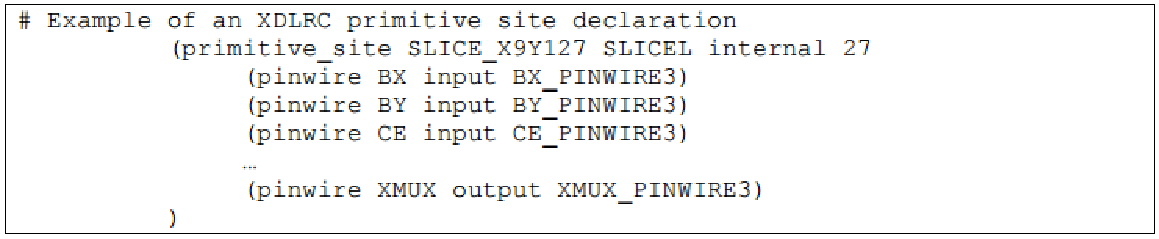
\includegraphics[width=1\columnwidth]{xdlrcSite}
	\caption{Primitive site syntax in XDLRC files}
	\label{fig:xdlrcSite}
\end{figure}

\noindent
Primitive site declarations in XDLRC files contain a list of pinwires which
describe the name and direction of pins on the primitive site. The first
pinwire declared in the example above is the BX input pin which is the internal
name to the SLICEL primitive site. Pinwires have an external name as well to
differentiate the multiple primitive sites that may be present in the same
tile. In this case, BX of SLICE\_X9Y127 has the external name BX\_PINWIRE3. In
RapidSmith, only the first pin name (i.e. BX above) is used.

\bigbreak \noindent
\begin{large}
\pgm{Wire}
\end{large}

\begin{figure}[H]
	\centering
	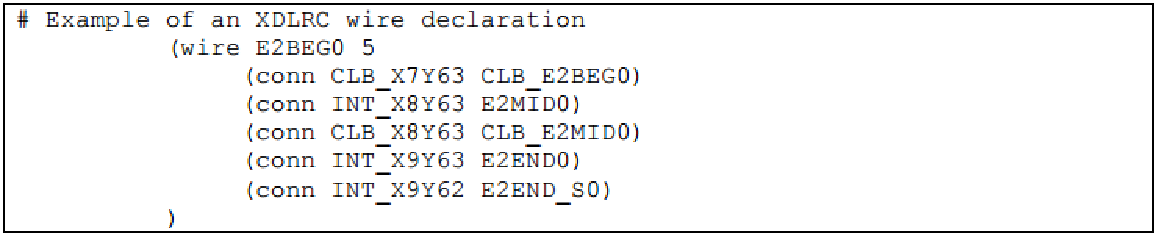
\includegraphics[width=1\columnwidth]{xdlrcWire}
	\caption{Wire syntax in XDLRC files}
	\label{fig:xdlrcWire}
\end{figure}

\noindent
A wire as declared in XDLRC is a routing resource that exists in the tile that
may have zero or more connections leaving the tile. In the example above, the
wire ``E2BEG0'' connects to 5 neighboring tiles. These connections (denoted
by ``conn'') are described using the unique tile name and wire name of that tile
to denote connectivity. The connections are not programmable, but hard wired
into the FPGA. Wire portions of the XDLRC file are included in the definition of
every tile (even if the same tile type has already been printed), which has a
big impact on the final size of XDLRC files. How RapidSmith handles wire
duplication is described in \autoref{wireEnum}. The \cls{WireConnection}
objects that are created from this part of the XDLRC are described in
\autoref{wireConnSection}.

\bigbreak \noindent
\begin{large}
\pgm{PIP}
\end{large}

\begin{figure}[H]
	\centering
	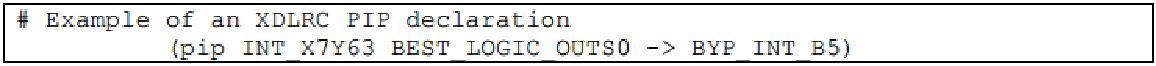
\includegraphics[width=1\columnwidth]{xdlrcPip}
	\caption{PIP syntax in XDLRC files}
	\label{fig:xdlrcPip}
\end{figure}

\noindent
A PIP (programmable interconnect point) is a possible connection that can be
made between two wires. In the example above, the PIP is declared in the tile
and repeats the tile name for reference. It specifies two wires by name that
both exist in that same tile (``BEST\_LOGIC\_OUTS0'' and ``BYP\_INT\_B5'') and
declares that the wire ``BEST\_LOGIC\_OUTS0'' can drive the wire
``BYP\-\_INT\_B5''. A collection of these PIPs in a net define how a net is
routed and is consistent with saying that those PIPs are “turned on.”
\autoref{wireConnSection} describes in detail how PIPs are represented in
RapidSmith.

\bigbreak \noindent
\begin{large}
\pgm{Primitive Definitions}
\end{large}

\bigbreak \noindent
The Primitive Definition portion of an XDLRC file textually describes the
components found within a \cls{Primitive} \cls{Site} type (a SLICEL for example)
and how they are connected. \cls{BEL}s, \cls{Site} \cls{Pins}, \cls{Site}
\cls{PIP}s, configuration options, and route-throughs are the elements that are
most commonly found within these parts of the file. An example of a complete
primitive definition file of type BUFHCE can be seen in
\autoref{fig:xdlrcDef}. The sub-site data structures in RapidSmith (\cls{Bels},
\cls{SiteWire}s, etc.) are built by parsing this section of the XDLRC file.

\begin{figure}[H]
	\centering
	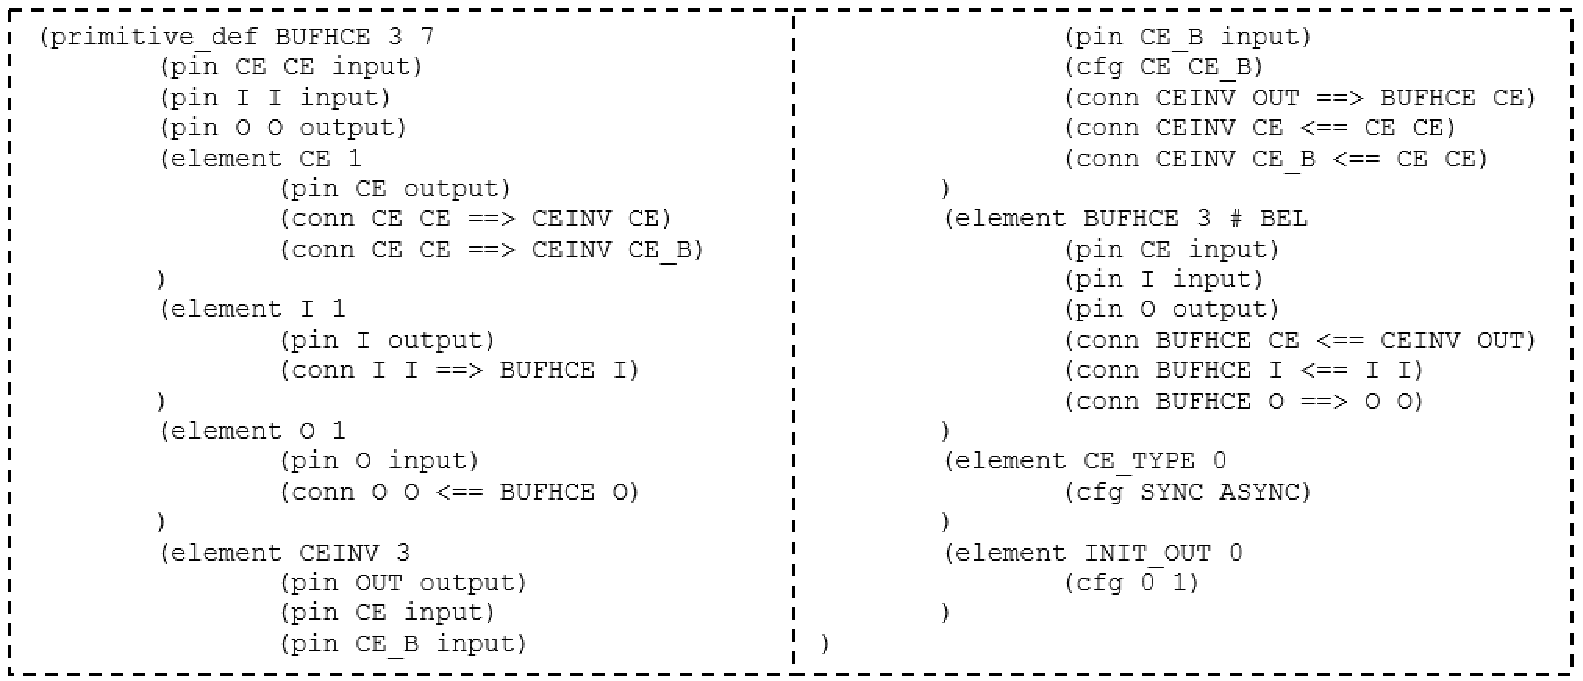
\includegraphics[width=1\columnwidth]{xdlrcDef}
	\caption{Primitive Def sections of XDLRC files}
	\label{fig:xdlrcDef}
\end{figure}

\pagebreak
\section{Designs in RS2}

\subsection{Xilinx Netlists} \label{sec:xilinxNetlist}
During the synthesis stage of implementation, a digital circuit expressed using
RTL (VHDL or Verilog) is translated to a lower level Xilinx netlist. This
netlist describes a digital circuit in terms of primitive elements that can
directly target hardware on a Xilinx FPGA. In terms of granularity, a Xilinx
netlist is more abstract than gates and transistors, but more detailed than RTL. A list of valid
primitives (also called \cls{Cell}s) that can be used within a Xilinx netlist
can be found
\href{http://www.xilinx.com/support/documentation/sw_manuals/xilinx2016_2/ug953-vivado-7series-libraries.pdf}{\color{blue}{here}}
for 7 Series devices and
\href{http://www.xilinx.com/support/documentation/sw_manuals/xilinx2014_1/ug974-vivado-ultrascale-libraries.pdf}{\color{blue}{here}}
for Ultrascale devices. It is suggested that users of RapidSmith become
familiar with the primitives found in these documents, and how they are used.
The primitives of a Xilinx netlist are wired together to create a digital
circuit (such as an 32-bit adder) capable of being implemented on an FPGA.
\autoref{fig:schematic} shows an example netlist of a 3-bit counter that has
been synthesized in Vivado. 

\begin{figure}[H]
 \centering
 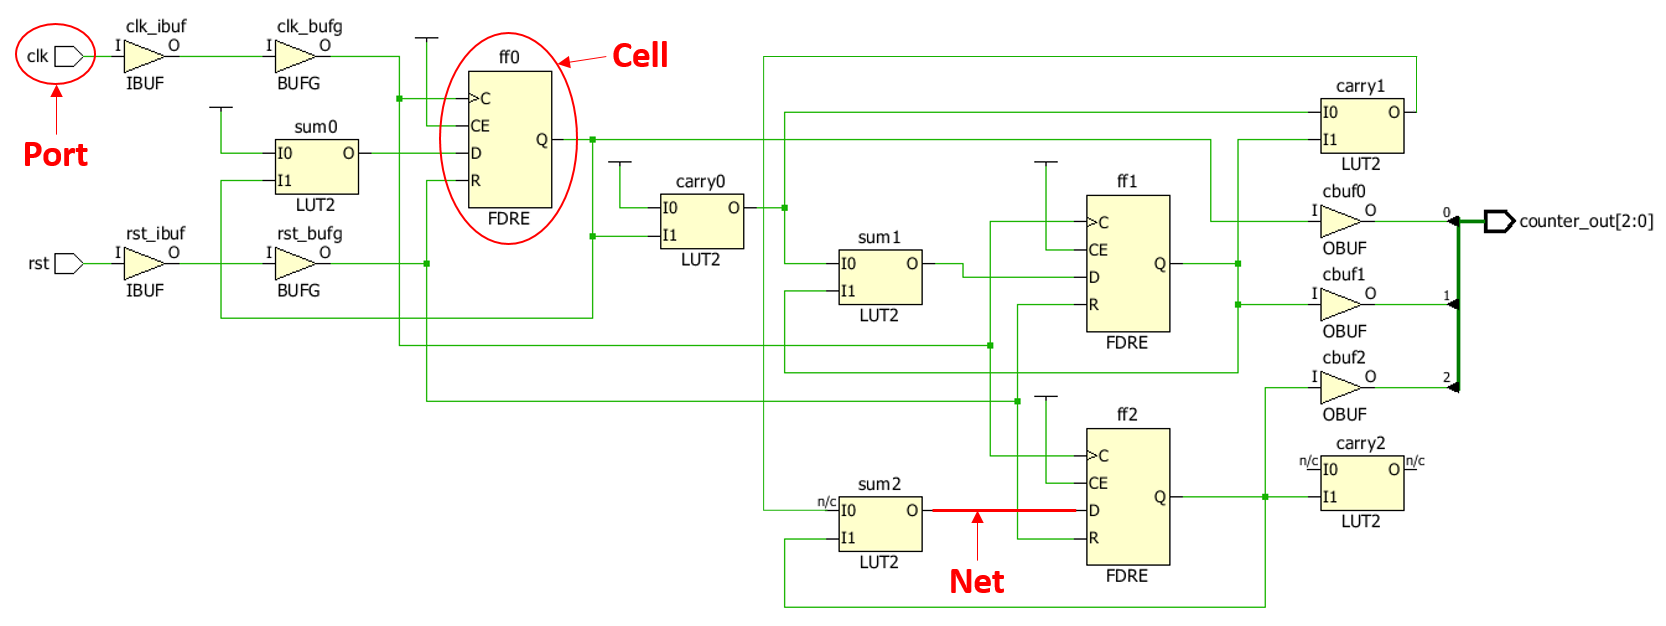
\includegraphics[width=1\columnwidth]{schematic.png}
 \caption{Schematic of a 3-bit counter in Vivado using LUT and FDRE cells.
 The yellow boxes are \cls{Cell}s, the green lines are \cls{Net}s, and and the
 white figures on the edge of the diagram are \cls{Port}s. An example of each
 of these netlist components have been highlighted.}
 \label{fig:schematic}
\end{figure}

As the figure shows, Vivado netlists are composed of three primary components:
\cls{Cell}s, \cls{Net}s, and \cls{Port}s. \cls{Cell}s are \pgm{instances} of
Xilinx primitives. They are the basic building blocks of a Xilinx netlist and
implement the actual logic of a digital design. The most commonly used
\cls{Cell}s include:

\begin{itemize}
  \item \pgm{Look Up Tables} (LUTs): Implement logic equations such as
  $O6 = (A1 + A2) \oplus A3$.
  \item \pgm{Flip Flops} (FDxx): Single-bit storage elements.
  \autoref{fig:schematic} uses an FDRE cell which specifies a rising-edge
  Flip Flop with a reset port, but ties the clock enable port high. Other
  types of FDxx cells can be used to include a clock enable signal (replace xx
  with the corresponding letters).
  \item \pgm{Block Ram} (BRAMs): On-chip FPGA memory cell.
  \item \pgm{Digital Signal Processing Units} (DSPs): Perform complex arithmetic
  functions efficiently.
  \item \pgm{Buffers} (BUF): IO, clock, and other types of signal buffers. 
\end{itemize}

\noindent
There exists several other types of \cls{Cell}s, but the ones in the list above
are the most prevalent. \cls{Net}s are used to connect \cls{Cell}s together. In
other words, the output of one \cls{Cell} is wired to the input of another
\cls{Cell} using a \cls{Net}. \cls{Port}s are simply design
Input/Output (IO). In terms of an FPGA design, \cls{Port}s are connected to
specific peripheral pins of the FPGA for chip IO. It is important to note that
a Xilinx netlist is purely logical, there is no physical information within the
netlist (i.e. there is not information about where the \cls{Cell}s have been
placed, or how the \cls{Net}s have been routed). When exporting a design from
Vivado, the Xilinx netlist representation is converted to EDIF. In order to
recreate the design in RapidSmith, the EDIF file is parsed and converted to a
custom netlist structure described in the next section.

\subsection {RS2 Netlist Data Structures} \label{sec:designDS}

RapidSmith netlists are modeled closely after Xilinx netlists. In fact,
much of the terminology between the two are identical or very similar. For those
that are familiar with Vivado designs, this should make the transition to
RapidSmith straightforward. The data structures that constitute a RapidSmith
netlist can be found in the package \pkg{byu.edu.ece.rapidSmith.design.subsite}.
The package hierarchy can be seen in \autoref{fig:designDS}.

\begin{figure}[H]
 \centering
 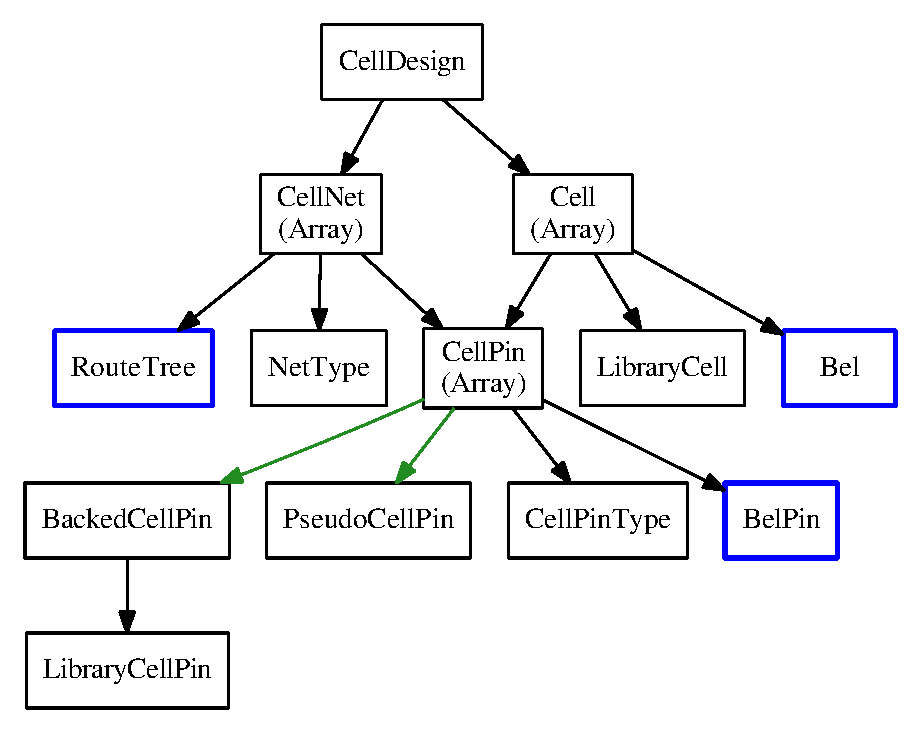
\includegraphics[width=.6\columnwidth]{designDS.eps}
 \caption{RapidSmith 2 design data structure tree. Black arrows represent
 composition (i.e. a \cls{CellDesign} contains an array of \cls{CellNet}s and
 an array of \cls{Cell}s). Green arrows represent inheritance (i.e. a
 \cls{CellPin} can be either a \cls{BackedCellPin} or a
 \cls{PseudoCellPin}). Blue boxes represent physical implementation components
 of the netlist (i.e. what physical \cls{Bel} a \cls{Cell} is placed on, or what
 physical \cls{Wire}s are used in a \cls{CellNet}).}
 \label{fig:designDS}
\end{figure}

\noindent
A \cls{CellDesign} is the top level design object in RapidSmith. It consists of
a collection of \cls{Cell} objects, interconnected by \cls{CellNet}s. RapidSmith
\cls{Cell}s are equivalent to Xilinx \cls{Cell}s and RapidSmith \cls{CellNet}s
are equivalent to Xilinx \cls{Net}s. \cls{Cell} objects have a template
\cls{LibraryCell}, which represents a Xilinx primitive. They also have a
collection of \cls{CellPin}s, which can be thought of as \cls{Cell} IO. 
During the placement phase of implementation, \cls{Cell}s may be mapped onto
\cls{BEL}s and the corresponding \cls{CellPin}s mapped onto \cls{BelPin}s.
Placement is described in more detail in \autoref{sec:placement}. \cls{CellNet}
objects connect \cls{Cell}s together via their \cls{CellPin}s.
During the routing phase of implementation, a \cls{CellNet} maps onto one or
more \cls{RouteTree}s. Routing is described in more detail in
\autoref{sec:routing}. The best way to learn how to use these classes is to read
through the \href{https://github.com/byuccl/RapidSmith2}{\color{blue}{Javadocs}}, but
important aspects of each class is included in the following subsections.


\subsubsection{\cls{CellDesign}}
As previously mentioned, the \cls{CellDesign} class is the top level netlist
structure. A Vivado design is converted from a Tincr checkpoint to a
\cls{CellDesign} on import, and converted from a \cls{CellDesign} to a Tincr
checkpoint on design export. It contains the following:

\begin{itemize}
  \item A list of uniquely named \cls{Cell}s in the design.
  \item A list of uniquely named \cls{CellNet}s in the design
  \item Global GND and VCC \cls{CellNet}s
  \item \cls{Cell} placement information (where each cell is placed)
  \item Internal routing configuration for each \pgm{used} \cls {Site} (in the
  form of \cls{Site} \cls{PIP}s)
  \item A list of XDC constraints imported from Vivado. See \autoref{sec:import}
  for more information about XDC constraints and how they are represented in
  RapidSmith.
\end{itemize}

\noindent
The \cls{CellDesign} class has a variety of methods to retrieve and manipulate
the \cls{Cell}s and \cls{CellNet}s of a design, place \cls{Cell}s onto
physical \cls{BEL}s, configure sub-site routing, and perform several other
tasks. See the
\href{https://github.com/byuccl/RapidSmith2}{\color{blue}{Javadocs}} for the
exact API.
 
\subsubsection{\cls{Cell}}
This section contains a few things you should know about \cls{Cell}s in, no
particular order.

\begin {itemize}
  \item A \cls{Cell} always contains a reference to a backing \cls{LibraryCell}.
  A \cls{LibraryCell} is equivalent to a Xilinx primitive cell (described in
  \autoref{sec:xilinxNetlist}), and serves as a template for instantiated
  \cls{Cell} objects. The template is used to save memory when creating several
  \cls{Cell}s of the same type. Whenever a new \cls{Cell} object is created, a
  corresponding \cls{LibraryCell} must be specified in the constructor. The
  method call \texttt{CellDesign.getCellsOfType(String,CellLibrary)} can be used
  to get all \cls{Cell}s in the current design with a specific \cls{LibraryCell}
  type.
  \item A \cls{Cell} has a list of \cls{CellPin}s that can connect to
  \cls{CellNet}s. The methods \texttt{Cell.getPins()},
  \texttt{Cell.getInputPins()}, and \texttt{Cell.getOutputPins()} can be used to
  get a handle to the pins of a \cls{Cell}. If more pins are
  needed on a \cls{Cell}, \cls{PseudoCellPin} objects can be attached (see
  \autoref{sec:cellPin}). \item \cls{Cell}s can be placed onto \cls{BEL}s of the
  current \cls{Device}. See \autoref{sec:placement} for more information about
  cell placement.
  \item Top-level \cls{Port}s in Vivado (design input/output) are represented as
  Port \cls{Cell}s in RapidSmith. Specifically, there are three types of port cells: IPORT, 
  OPORT, and IOPORT. The method \texttt{CellDesign.getPorts()} can
  be used to iterate through the port \cls{Cell}s in a design, and the method
  \texttt{Cell.isPort()} can be used to determine if a given \cls{Cell} is
  actually a port.
\end{itemize}

\subsubsection{\cls{CellPin}} \label{sec:cellPin}

There are two types of \cls{CellPin} objects in RapidSmith:
(1) \cls{BackedCellPin}s and (2) \cls{PseudoCellPin}s. \cls{BackedCellPin}s are
straightforward. They represent a \cls{LibraryCellPin}, which is a pin attached
to the corresponding \cls{LibraryCell} of a \cls{Cell}. These pins are used as
signal input and signal output. On the other hand, \cls{PseudoCellPin}s are
``fake" \cls{CellPin} objects which are added to a \cls{Cell} after
the \cls{Cell} has been created. They don't affect the functionality of the
\cls{Cell}, but are needed for physical implementation. An example of where a
\cls{PseudoCellPin} is needed can be seen in \autoref{fig:pseudoPin}.

\begin{figure}[H]
 \centering
 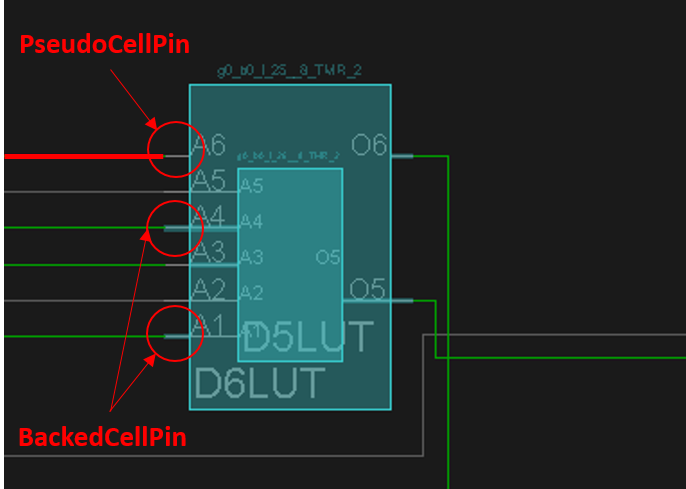
\includegraphics[width=.5\columnwidth]{pseudoPin.png}
 \caption{An example where a \cls{PseudoCellPin} in RapidSmith may be needed.
 Both a \cls{PseudoCellPin} and \cls{BackedCellPin} are pointed out. The red net
 in the image (going into the A6 pin) is the power net (VCC).}
 \label{fig:pseudoPin}
\end{figure}

\noindent
In the figure, a cell of type LUT2 has been placed onto a D6LUT \cls{BEL} of a
SLICEL. The two \cls{CellPin}s of the LUT2 have been mapped to the A1 and A4
pins of the \cls{BEL} (which have been highlighted in blue), connected to
\cls{Net}s, and routed. This is expected behavior based on the netlist.
Also, the global VCC net has been routed to the A6 \cls{BelPin}. This is
necessary due to the hardware implementation of LUTs. However, in the
netlist view of the circuit, the fact that VCC needs to be routed to the A6 pin
is not at all represented (a \cls{CellNet} can only be connected to
\cls{CellPin}s). This is where \cls{PseudoCellPin}s are helpful.
In RapidSmith, a \cls{PseudoCellPin} can be added to the LUT2 cell (called
``VCCPin''), mapped to the A6 \cls{BelPin}, and attached to the global VCC
\cls{CellNet}. This gives a more complete view of how the netlist needs to be
physically implemented. \cls{PseudoCellPin}s are created and added
automatically to \cls{Cell}s when importing a Tincr checkpoint. If you are
creating \cls{Cell}s from scratch, a \cls{PseudoCellPin} can be added with the
method call \texttt{Cell.attachPseudoPin(string,PinDirection)}. To determine if
a \cls{CellPin} is a \cls{PseudoCellPin}, the method call
\texttt{CellPin.isPseudoPin()} can be used. That
being said, in general \pgm{users do not need to worry about the different
between pseudo and backed \cls{CellPin}s} when creating a CAD algorithm. They
function identically, so you can use the higher level handles to the
\cls{CellPin} interface instead.

Each \cls{CellPin} object also has a \cls{CellPinType} and \cls{PinDirection}
enumeration. \autoref{tab:pinEnums} displays the possible values for both of
these enumerations. The \cls{CellPinType} field can be used to find all RESET
\cls{CellPin}s in a design, determine if a \cls{CellNet} is a clock net (it
connects to pins of type CLOCK), and other useful functions. The
\cls{PinDirection} field is typically used to filter a list of \cls{CellPin}s by
their direction. It it especially useful in determining if a pin on a \cls{Cell}
is of type INOUT. 

\begin{table} [h!]
\begin{center}
\begin{tabu}{ |c|l| }
%\begin{tabular}{ |p{2cm}|p{3cm}| }
\hline
\pgm{Enum} & \multicolumn{1}{|c|}{\textbf{Values}}\\
%\pgm{Enum} & \textbf{Values} & \textbf{Description} \\
\hline
\hline
 & CLEAR \\ 
 & CLOCK  \\
 & ENABLE \\      
 & PRESET \\ 
 & RESET \\
\cls{CellPinType} & REUSED \\
 & SET \\
 & SETRESET \\
 & WRITE\_ENABLE \\
 & DATA \\
 & PSEUDO \\
\hline
 & IN \\
\cls{PinDirection} & OUT \\ 
 & INOUT\\ 
\hline
\end{tabu}
\caption{Enumerations for the \cls{CellPin} class}
\label{tab:pinEnums}
\end{center}
\end{table}

\subsubsection{\cls{CellNet}}
\cls{CellNet}s are used to wire components of a logical netlist
together. Specifically, a \cls{CellNet} connects an output
\cls{CellPin} to several input \cls{CellPin}s with the purpose of transferring
a signal from one \cls{Cell} to another. The remainder of this section details
important aspects about \cls{CellNet}s in RapidSmith.

\begin{itemize}
  \item \cls{CellNet}s are routed using the \cls{RouteTree} data structure.
  Routing in RapidSmith is described in more detail in \autoref{sec:routing}.
  \item All \cls{CellNet}s have a \cls{NetType} enumeration. Possible values for
  \cls{NetType} include VCC, GND, and WIRE. VCC is reserved for power nets, GND
  is reserved for ground nets, and WIRE represents all other nets in the design.
  Other \cls{NetType}s could be added to this list in the future (such
  as CLOCK), but for now they are not differentiated.
  \item VCC and GND nets (also called static nets) are treated specially in
  RapidSmith in two ways. (1) Vivado designs can have multiple nets that
  correspond to VCC or GND, but they all logically represent the same thing.
  This representation can be challenging to work with when designing CAD tools.
  RapidSmith takes a different approach. When a design is imported from Vivado,
  all VCC nets are collapsed into a single VCC net that is sourced by a global
  VCC cell (the same applies to GND nets). We have found this representation
  much easier to work with. The function calls \texttt{CellDesign.getVccNet()}
  and \texttt{CellDesign.getGndNet()} can be used to retrieve these special
  nets from the design. If you add a VCC net to a design that already has a VCC
  net, the old net will be overridden. (2) When a static net is routed, it
  doesn't have a single source driving it. Rather, the net is partitioned
  into sections with each section having a single source. In an FPGA, each of
  these sources corresponds to a TIEOFF within a switchbox tile. This is shown
  in \autoref{fig:staticNetSources}.
  
  \begin{figure}[H]
   \centering
   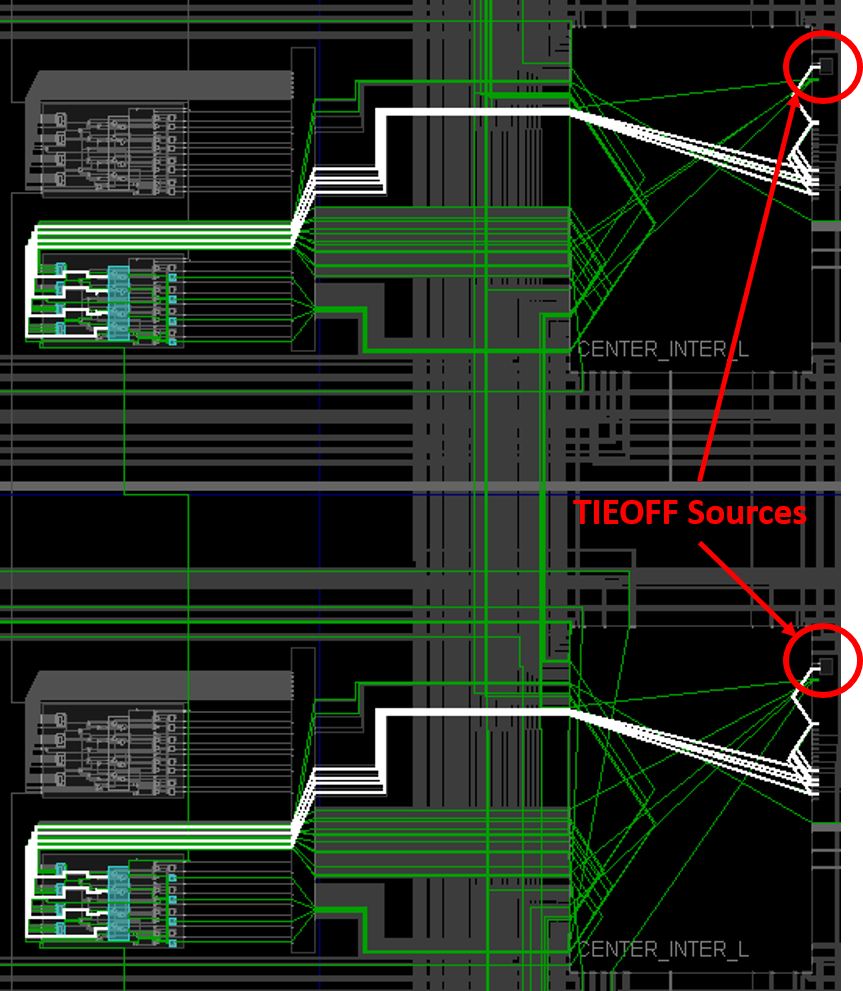
\includegraphics[width=.5\columnwidth]{staticNetSources.png}
   \caption{Static net multiple sources example. The higlighted white wires are
   a part of the same GND net, and the circled red areas are the source TIEOFFs
   for the GND net. In this image, only two sources are shown.}
   \label{fig:staticNetSources}
  \end{figure}
  
  RapidSmith handles this oddity by allowing \cls{CellNet}s to have more than
  one RouteTree object associated with it. In the case of
  \autoref{fig:staticNetSources} the GND net would have two \cls{RouteTree}
  objects associated with it, one for each source TIEOFF.
   
  \item Most \cls{CellNet}s have a single source pin and multiple sink pins
  (referred to as the ``fanout'' of the net). When routing a net that fits
  this description, only one RouteTree needs to be specified. However, there are
  two noticable exceptions to the common case: (1) static nets (described
  in the bullet point above) and (2) nets with multiple drivers (involving IO
  pins). In a Xilinx FPGA, this is most often seen in IOB pads. An example is
  shown in \autoref{fig:iobNet}. The highlighted net can be driven by both the OBUF output, and from an
  external source. RapidSmith 2 supports nets with multiple drivers. The
  function call \texttt{CellNet.getAllSources()} can be used to retrieve all
  possible source \cls{CellPin}s of a net.
  
  \begin{figure}[H]
   \centering
   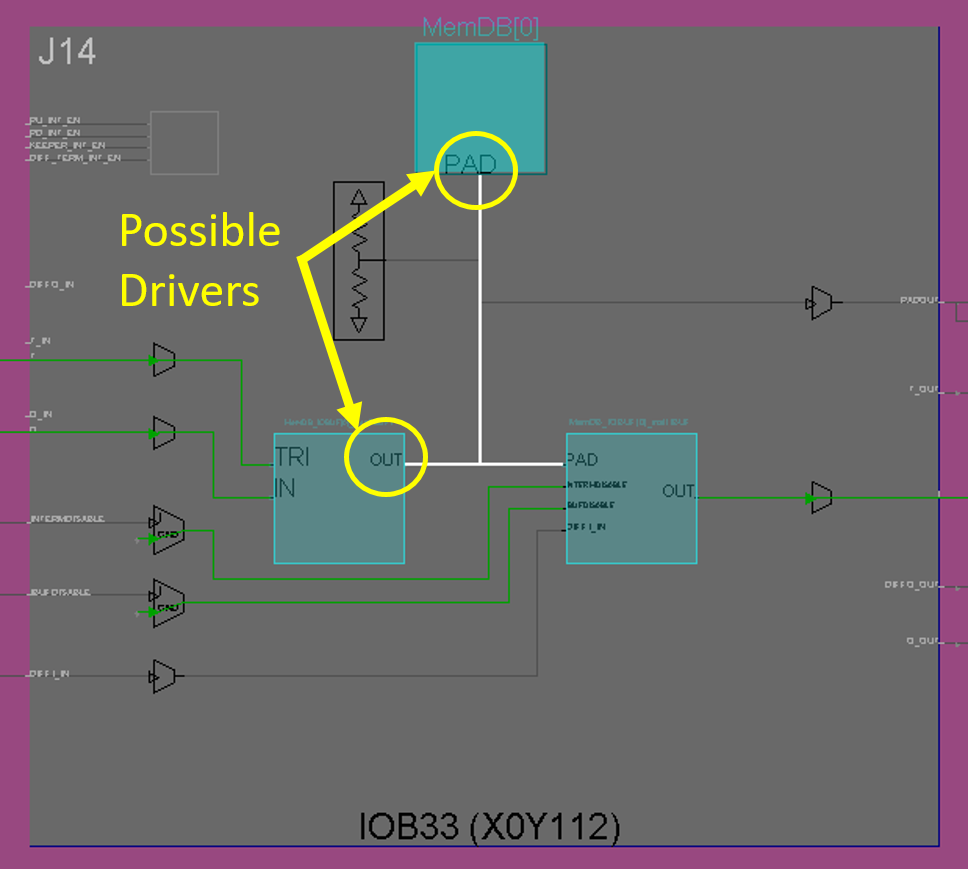
\includegraphics[width=.5\columnwidth]{iobNet.png}
   \caption{An example of net (highlighted in white) that can be driven by more
   than once source.}
   \label{fig:iobNet}
  \end{figure}
  
  \item After a design has been placed, \cls{CellNet}s fall into one of two
  categories: INTRASITE or INTERSITE. \autoref{fig:interVsIntra} shows an
  example of both types of nets. As can be seen, INTRASITE nets do not cross
  \cls{Site} boundaries while INTERSITE nets stretch across multiple
  \cls{Site}s. These types of nets are handled differently during routing. To
  determine if a \cls{CellNet} is an INTRASITE net, the method call
  \texttt{CellNet.isIntrasite()} can be used.
  
  \begin{figure}[H]
   \centering
   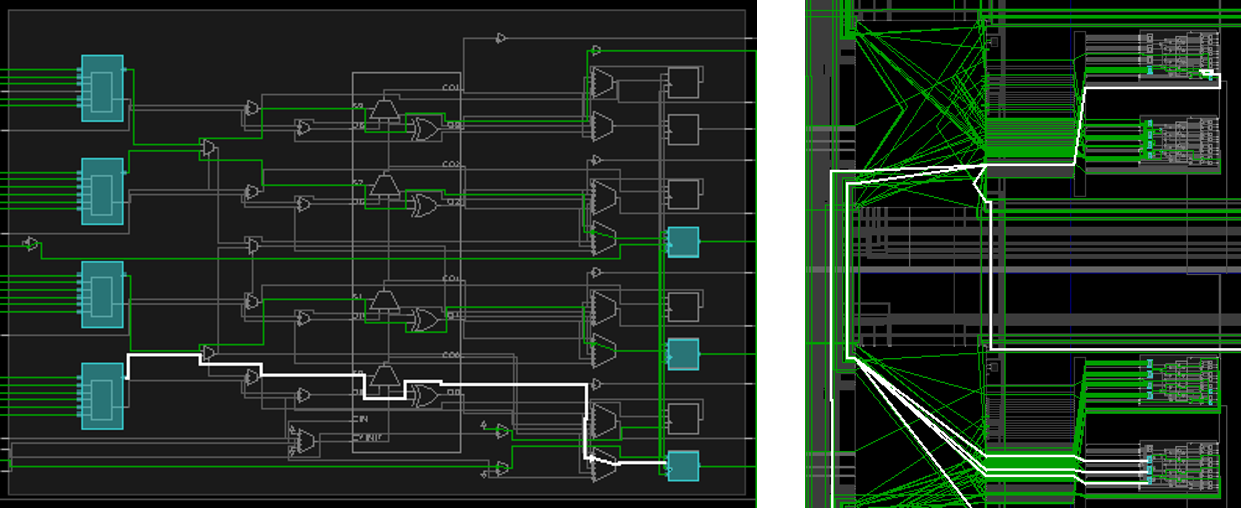
\includegraphics[width=.9\columnwidth]{interVsIntra.png}
   \caption{Example of an INTRASITE net (left) and an INTERSITE net (right).}
   \label{fig:interVsIntra}
  \end{figure}
  
\end{itemize}

\subsubsection {\cls{PropertyList}}

In Vivado the top-level design, cells, and nets all have properties associated
with them. The Tcl command \texttt{[report\_\-property \$object]} can be used to
view the properties of a Vivado Tcl object. When a design is exported from
Vivado, these properties (\pgm{if they are not the default value}) are stored
in the EDIF netlist file. When RapidSmith parses the EDIF file, the properties
are stored in a data structure called a \cls{PropertyList}. Each
\cls{CellDesign}, \cls{Cell}, and \cls{CellNet} in RapidSmith has an associated
\cls{PropertyList} object, which can be retrieved using the method
\texttt{getProperties()}. \cls{PropertyList} implements the \cls{Iterable}
interface, so properties of an object can be iterated through easily using a
for-loop. Also, properties can be retrieved by their string name. Because EDIF
properties only support String, Integer, and Boolean types, any properties
imported from Vivado will have one of these types.
	
\cls{Cell}s are the most interesting objects
in terms of properties. This is because the function of a \cls{Cell} is
determined by how it is configured. For example, the memory width of a BRAM cell
in Vivado is configured by setting the ``READ\_WIDTH'' and ``WRITE\_WIDTH''
properties. Possible values include 1, 2, 4, 9, 18, 36 and 72. Another example
is a D flip flop cell (FDRE) and its ``CONFIG.INIT'' property. This property
indicates what the flip flops power-up state should be. Some additional things
about cell properties that may be helpful include:

\begin{itemize}
  \item To learn what configuration properties a \cls{Cell} has, open up a
  Vivado design and type the following into the console,
  
  \begin{code}
  Vivado\% link_design -part xc7a100tcsg324-3 -quiet
  Vivado\% set lib_cell [get\_lib\_cells RAMB36E1]
  Vivado\% report_property \$lib_cell 
  \end{code}
  
  replacing ``xc7a100tcsg324-3'' with the part you are using and ``RAMB36E1'' with your
  cell of interest. All properties that start with ``CONFIG'' represent
  configuration properties that a user can set.
  \item To learn what configuration properties \pgm{affect the pin mappings of
  a cell}, open the \fil{cellLibrary.xml} file you have, and search for the
  tag ``libcellproperty.'' Pin mappings are described in more detail in
  \autoref{sec:placement}.
  \item Only properties of type EDIF will be exported from RapidSmith. If you
  create cells in your design and add properties to them, make sure that you
  mark the properties as EDIF properties by setting their type. All other
  properties will be ignored.
  \item Some properties not only affect how a \cls{Cell} is configured, but they
  can also affect how a \cls{Site} is configured. For example, on SLICEL
  sites there exists a clock routing mux that chooses between a regular clock
  signal and an inverted signal. This inverter is connected to the flip flops of
  the SLICEL, and so decides whether the flip flops are rising-edge or falling-edge
  triggered. The clock that is selected is decided by the property
  ``CONFIG.IS\_C\_INVERTED'' of the flip flops cells \pgm{that have been placed
  on the SLICEL}. The clock inverter is programmed automatically based on the
  cell properties. There are other such properties, but they will not be
  listed here. When creating designs in RapidSmith, it is important to not
  place \cls{Cell}s together that may have conflicting properties. RapidSmith
  does not perform any error checking, and so an error in Vivado will be thrown
  if you violate property restrictions.
\end{itemize}

\subsection{The Cell Library}

The \cls{CellLibrary} in RapidSmith stores important information about each of
the \cls{LibraryCell}s compatible with a specific Xilinx FPGA part.
This includes: 

\begin {itemize}
  \item The name of the library cell
  \item The name, direction, and type of each library cell pin
  \item Valid placement locations for instances of the library cell
  \item Possible logical-to-physical pin mappings for every library pin
  \item Configuration properties of the library cell (TODO)
\end{itemize}

\noindent
When doing any type of netlist modification, the \cls{CellLibrary} is needed.
Currently, each \cls{CellLibrary} corresponds to a specific Xilinx
part.
This means that for each part you use in RapidSmith, a new \cls{CellLibrary}
needs to be generated \footnote{This may change to be family-specific in the
future. Usually, parts in the same family can use the same
\cls{CellLibrary}. The part-specific mention is very conservative, but is one
that we know is right}.
The rest of this section demonstrates how to get access to a cell library in
RapidSMith, and how to create a new cell library XML file from Tincr.

\subsubsection{Getting a handle to the Cell Library}
When a Tincr checkpoint is imported into RapidSmith, a \cls{CellLibrary} is
automatically loaded. To get a handle to the \cls{CellLibrary}, you can use
the method call \texttt{TincrCheckpoint.getLibCells()} on the Tincr checkpoint
object that was loaded. If you only have a handle to a \cls{Device} object, then
the code below can be used to load a cell library from disk:

\begin{code}
CellLibrary libCells = new CellLibrary(RSEnvironment.defaultEnv()
                       .getPartFolderPath(device.getPartName())
                       .resolve(CELL_LIBRARY_NAME));
\end{code}

\subsubsection{Generating a new Cell Library}
During runtime, a \cls{CellLibrary} data structure is created by parsing a
\textit{cellLibrary.xml} file into memory. So, to create a new \cls{CellLibrary}
all you have to do is generate a new \textit{cellLibrary.xml} file for the
Xilinx part you are interested in. This can be done in a few easy steps.

\begin{enumerate}
  \item Open Vivado in Tcl mode, and type the following into the console:
  \begin{code}
::tincr::create_xml_cell_library xc7a100tcsg324-3 mycellLibrary.xml
  \end{code}
  Replace ``xc7a100tcsg324-3'' with the part you want to generate and
  ``mycellLibrary.xml'' with the location where you want to store the generated
  cell library XML. This will generate most of what you need in the cell library
  XML automatically.
  \item Open the generated XML file in a text editor and search for the
  ``CARRY'' cell (could be the CARRY4 or CARRY8).
  \item Scroll down to the ``bels'' XML element within the CARRY cell,
  and add the following lines to each pin that is named ``CI'':
  
  \begin{figure}[H]
   \centering
   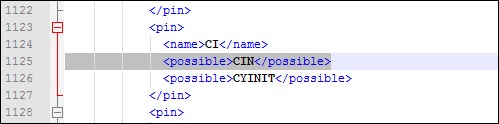
\includegraphics[width=.9\columnwidth]{cellLibHandEdit.png}
   %\caption{Example of an INTRASITE net (left) and an INTERSITE net (right).}
   %\label{fig:interVsIntra}
  \end{figure}
  
  If the cell is a CARRY4, you should have to insert this line in two places
  only.
  \item Save your changes and exit the text editor
  \item Copy the XML file to \textit{\$RapidSmith\_Path/device/family}
  directory where ``family'' is replaced by the family of your part (such as
  Artix7), and ``\$RapidSmith\_Path'' is your RapidSmith repository location.
  Once this is done the new \cls{CellLibrary} should be ready to use. 
\end{enumerate}

\pgm{NOTE}: Usually, parts in the same family can use the same
\cls{CellLibrary}.


\pagebreak
\section{Placement in RS2} \label{sec:placement}

In the original RapidSmith, placement occurred at the \cls{Site} level. A
collection of \cls{Cell}s were grouped together in what was called an
\cls{Instance}, and the \cls{Instance} was assigned to a compatible site type.
Where the individual \cls{Cell}s were actually placed within the \cls{Site}
was a blackbox. Because RapidSmith 2 breaks up a \cls{Site} into its
individual components, \cls{Cell}s can now be placed directly onto
physical \cls{BEL}s within a \cls{Site}. This gives Xilinx FPGA CAD developers
finer grain control during the placement of a design, and allows sub-site
algorithms (such as packing algorithms) to be explored. \autoref{code:place}
demonstrates the basic steps to placing a \cls{Cell} in RapidSmith.

\begin{lstlisting} [caption=Steps for placing a Cell in RapidSmith,label=code:place]
// Load the device and design
TincrCheckpoint tcp = VivadoInterface.loadTcp("myCheckpoint.tcp"); 
Device device = tcp.getDevice();
CellDesign design = tcp.getDesign();

// Get a handle to a Cell and Bel. The cell is of type LUT2 
Cell cell = design.getCell("MyCell"); 
Bel bel = device.getSite("SLICE_X40Y137").getBel("D6LUT");

// Place the cell onto the bel
design.placeCell(cell,bel);

// Two ways to map bel pins
CellPin pin1 = cell.getPin("I0");
CellPin pin2 = cell.getPin("I1");
CellPin pin3 = cell.getPin("O")

// First way
pin1.mapToBelPin(bel.getPin("A1"));
pin2.mapToBelPin(bel.getPin("A2"));

// Second way
List<BelPin> possible = pin3.getPossibleBelPins(bel);
pin3.mapToBelPin( possible.get(0) );
\end{lstlisting}

\noindent
As the code listing shows, there are two steps to placing a RapidSmith
\cell. The first is straightforward: get a handle to a \bel object,
and use the method call \texttt{CellDesign.placeCell(Cell, Bel)} (line 11). This
will map a logical \cell onto a physical \bel. Once a \bel has been
used, no other \cells can be mapped to it. No error checking is performed to
ensure that a \cell is compatible with the \bel it is being placed on, that is
up to the user. The second step is more complicated: each logical \cellpin of
the \cell needs to be mapped to a physical \belpin. This can be done by
either (a) specifying the \belpin name (lines 19-20), or (b) using
the function call \texttt{CellPin.getPossibleBelPins(Bel)} (line 23) to
get a list of valid \belpin mappings. For most \cells each \cellpin only
maps to a single \belpin, and so option (b) is preferable. However, there are two
noticable exceptions to this rule.

\begin {enumerate}
  \item LUT input pins are permutable. This means that an input \cellpin 
  attached to a LUT \cell can be mapped to any input pin of a LUT \bel.
  \autoref{fig:lutPins} shows an example of this functionality in Vivado. Once
  the input pins have been mapped, a configuration equation is created for and
  applied to the LUT \bel using the appropriate \belpin inputs.
  In order for a LUT \cell to be physically implemented, these pins need to be
  mapped. The function call \texttt{CellPin.getPossibleBelPins(Bel)} in this
  case will return all of the input \belpins of the LUT and the user can decide
  which ones to use.
  
  \begin{figure}[t]
	\centering
	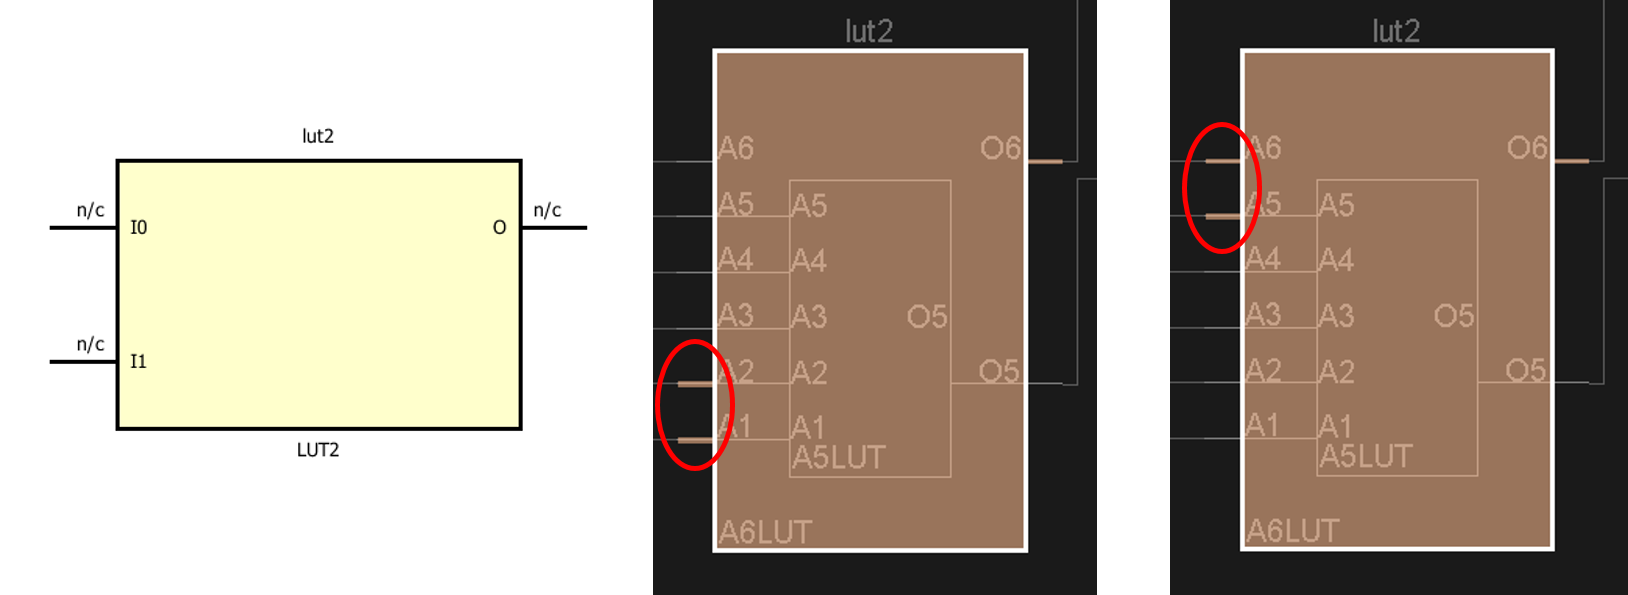
\includegraphics[width=1\columnwidth]{lutPins.png}
	\caption{An example of LUT pin permutations. The left figure shows the
	schematic of a LUT2 cell. The middle figure shows the two input pins of the LUT
	cell being mapped to the A1 and A2 pins of a LUT6 bel. The right figure shows
	the same input pins being mapped to the A6 and A5 pins instead.}
	\label{fig:lutPins}
  \end{figure}
  
  \item Logical-to-physical pin mappings can change \pgm{based on how a cell is
  configured}. For example, on a RAMB36E1 \cell, the least-significant data
  input pins map to different physical \belpins when the width of the BRAM is
  set to 72. This is an important concept when performing netlist modifications
  in RapidSmith. The function call \texttt{CellPin.getPossibleBelPins(Bel)} only
  returns the pin mappings for the \pgm{default} \cell configuration. The
  correct pin mappings are always used when a Tincr checkpoint is imported into
  RapidSmith, but if new logic is being added to a design it is up to the
  user to determine the proper pin mappings. Adding support for
  automatically determining a \cells pin mappings based on a its
  configuration is currently being worked on, but is not yet ready. For now,
  users can configure a cell in Vivado, place it, and use the TCL function shown
  in \autoref{code:tclPinMap} to determine the correct pin mappings for a \cell.

\end{enumerate}

\begin{lstlisting}[language=tcl, caption=TCL script to print all
logical-to-physical pin mappings of a cell,label=code:tclPinMap]

proc print_pin_mappings{cell} {

	foreach cell_pin [get_pins -of $cell] {
		puts "$cell_pin -> [get_bel_pins -of $cell_pin]" 
	}
}

\end{lstlisting}
 
\vspace{.2cm}
\noindent
Some additional points about placement to be aware of include: 

\begin {itemize}
  \item VCC and GND \cells are not placed when implementing a design in Vivado.
  This distinction is applied to RapidSmith 2 as well. Rather than placing VCC
  or GND explictly, \cls{RouteTree}s that are sourced by switchbox TIEOFFs are
  used to express their placement implicitly (VCC/GND is ``placed'' on the
  TIEOFF).
  \item A list of valid placement options for a \cell can be obtained with the
  function call \texttt{Cell.getPossible\-Anchors()}. The sample program
  \pgm{CreateDesignExample} (described in \autoref{sec:createDesignExample})
  gives a good example of how to use this function. The reader is referred to
  the source code and Javadocs for more details.
  \item If you plan on writing a placer in RapidSmith, there are several
  placement rules for a given device. A few examples include (a) CARRY4 \cells
  that are connected through the carry chain need to placed vertically to one
  another so they can use the dedicated carry wires, and (b) A RAMB36E1 cell
  cannot be placed in the same tile as a RAMB18E1 cell. If either of these
  rules are violated, an error will be thrown in Vivado. It is the
  responsibility of the user to determine all relevant placement rules
  because error checking is not performed on design export. The source code for
  a sample simulated annealing placer for the Artix-7 part {\em
  xc7a100tcsg324} can be found in the package
  \pkg{edu.byu.ece.rapidSmith.examples.placerDemo}.
\end{itemize}

\pagebreak
\section{Routing in RS2} \label{sec:routing}
After placement, all \cells of a design have been mapped to \bels, and their
corresponding \cellpins mapped to \belpins. The next (and final) step of the
FPGA implementation flow is to physically wire together the used \belpins. This
is known as routing. Routing involves taking each logical \net of a design,
determining the \belpins they are connected to (based on the \cellpins), and
finding a list of physical wires that electrically connect the pins together.
This section details how routing is done in RS2.

\subsection{Wires and WireConnections} \label{wireConnSection}
Routing in RapidSmith is done using \cls{Wire} objects, which are described in
\autoref{wireSection}. \cls{Wire}s are uniquely identified by their
corresponding tile and wire name (i.e. tile1/wire1), and are connected through
\cls{WireConnection} objects. There are two types of wire connections:

\begin {enumerate}
  \item \pgm{PIP Connections}: Connect two different wires through a
  Programmable Interconnect Point. Most PIP connections are found in
  switchbox tiles of an FPGA part (as shown in \autoref{fig:switchboxPIP}).
  These types of connections are important to FPGA routing, because they
  dynamically configure the routing network for a given design.
   
  \item \pgm{Non-PIP Connections}: Connect the same physical wire across two
  different tiles. In general, wires stretch across multiple tiles in a device, having
  a different name in each tile. This is demonstrated in
  \autoref{fig:wireFigure}. The example wire shown in the figure spans 5
  different tiles, but has a different name in each. To save space, only the
  source and sink wire segments are kept in RapidSmith data structures
  (\texttt{INT\_X1Y1/E2BEG4}, \texttt{INT\_X2Y1/E2MID4}, and
  \texttt{INT\_X3Y1/E2END4}). The source segment is connected to each sink
  segment through a non-PIP wire connection. It is also possible to have non-PIP
  connections within a \tile, but this is rare.
\end{enumerate} 

\begin{figure}[H]
\centering
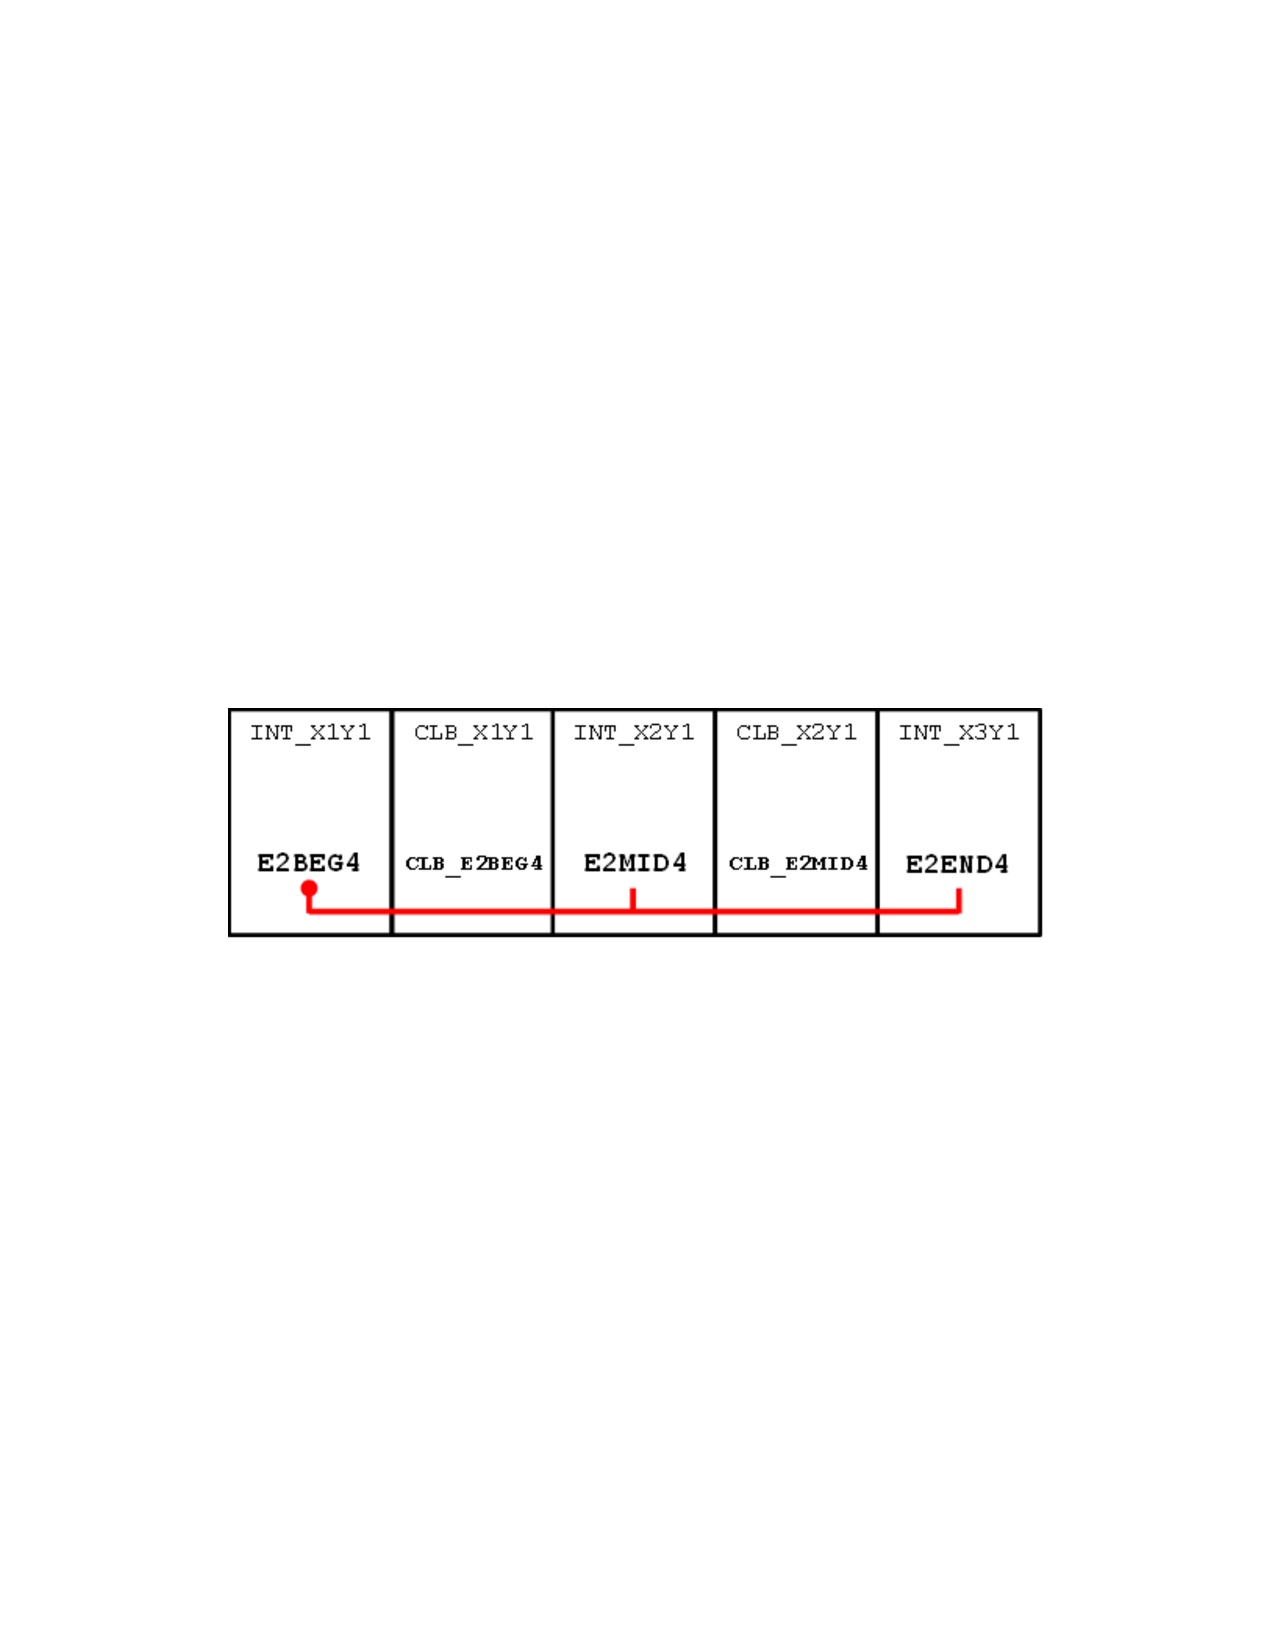
\includegraphics[width=0.8\columnwidth]{wireFigure}
\caption{A wire in an FPGA illustrating how each part of the wire has a
different name depending on the tile it is located in}
\label{fig:wireFigure}
\end{figure}

\subsection{Traversing Wire Objects}
Traversing through wires in a device is straightforward. Given a handle to a
\cls{Wire} object named "mywire" or a \cls{WireConnection} object named
"wc", the following function calls can be used:

\begin {itemize}
  \item \texttt{mywire.getWireConnections()}: Returns a collection of all
  \cls{WireConnection}s with the source wire of mywire. This collection can be
  iterated through to find all places a specific wire goes (i.e. what wires it
  connects to).
  \item  \texttt{wc.isPip()}: Returns true if the wire connection ``wc'' is a PIP
  connection. Returns false otherwise.
  \item \texttt{wc.getSinkWire()}: Returns the sink wire of a wire connection.
\end{itemize} 

\noindent
In general, these are the only three functions that are needed to
search through the wires of a FPGA device. It is important to note however that
the first wire in the route has to be either (a) created using a \cls{TileWire}
constructor, or (b) retrieved from a function call of another object (such as
\texttt{SitePin::getExternalWire()}). \autoref{code:connections} demonstrates
how to iterate through \cls{WireConnection} objects. To gain a better
understanding of how to use \cls{Wire}s and \cls{WireConnection}s, see the
\pgm{HandRouter} example in the RapidSmith repository.

\subsection{Other Types of Connections} \label{otherConns}
Along with PIP and non-PIP wire connections, there are several other types of
connections in RapidSmith. The source of the connection is always a \cls{Wire}
object, but the sink object differs. A description of these connections is found
below:

\begin {itemize}
  
  \item \pgm{Site Pin Connections}: Connects a \cls{Wire} to a \cls{SitePin}.
  The function call \texttt{conn.get\-SitePin()} can be used to get the sink
  \cls {SitePin} object.
  \item \pgm{Terminal Connections}: Connects a \cls{Wire} to a \cls{BelPin}. The
  function call \texttt{conn.get\-BelPin()} can be used to get the sink \cls
  {BelPin} object.
  \item \pgm{Site Routethrough Connections}: Connects an input site \cls{Wire}
  to an output site \cls{Wire}. A \cls{Site} in Vivado can be configured to pass
  the signal on an input \cls{SitePin} directly to an output \cls{SitePin}.
  These connections are represented as routethroughs in RapidSmith and can be
  determined with the function call \texttt{conn.isRoutethrough()}.
  \pgm{NOTE}: Before using this type of connection when building a
  routing data structure, make sure the \cls{Site} is unused.
  \item \pgm{BEL Routethrough Connections}: Connects an input BEL \cls{Wire} to
  an output BEL \cls{Wire}. Similarly to a \cls{Site} routethrough, LUTs in
  Vivado can also be configured as routethroughs. In this case, the signal on one of the
  input pins of the LUT is passed directly to the output pin of the LUT. A BEL
  routethrough connection can be used to configure a LUT as a routethrough in
  RapidSmith.
  \pgm{NOTE}: Before using this type of connection, make sure the LUT is
  unused (i.e. no cell is placed on it).
\end{itemize}

\noindent
When traversing through the device data structure, a generic \cls{Connection}
object is usually used. This connection can refer to any of the connections
described so far in this documentation. \autoref{code:connections} demonstrates
how to iterate through different \cls{Connection} types in RapidSmith.

\begin{lstlisting}[caption=How to iterate over Connections in RapidSmith,
label=code:connections] 
// Get a handle to a wire
Wire wire = sitePin.getExternalWire();

// Iterate over all WireConnections
for (Connection conn : wire.getWireConnections()) {
	Wire sinkWire = conn.getSinkWire();

	if (conn.isPip()) {
		// Do something with a PIP
	} 
	else if (conn.isRoutethrough()) {
		// Do something with a routethrough
	} 
	else {	
		// Do something with a regular wire connection				
	}
}

// Iterate over all Pin Connections
for (Connection conn : wire.getPinConnections() ) {
	SitePin pin = conn.getSitePin();
	// Do something with the SitePin
}

// Iterate over all Terminal Connections
for (Connection conn : wire.getTerminals()) {
	BelPin bp = conn.getBelPin();
	// Do something with the BelPin
}

// Iterate over all connections at the same time
Iterator<Connection> connIt = wire.getAllConnections().iterator();

while (connIt.hasNext()) {
	Connection conn = connIt.next();
	
	if (conn.isPinConnection()) {
		//do something with the site pin
	}
	else if (conn.isTerminal()) {
		//do something with the bel pin 
	}
	else if (conn.isPip()) {
		//do something with the pip wire connection
	}
	else {
		//do something with regular wire connection.
	}
}
\end{lstlisting}

\subsection{RouteTrees}

\cls{Wire}s and \cls{WireConnection}s are the fundamental objects used to
specify and explore routing in RapidSmith, but they need to be organized in
a higher-level data structure to give meaning to the route of a \cls{CellNet}.
In the original RapidSmith, creating this data structure was up to the user.
RapidSmith 2 introduces the \cls{RouteTree}, which can be see in
\autoref{fig:routeTreeDS}.

\begin{figure}[H]
\centering
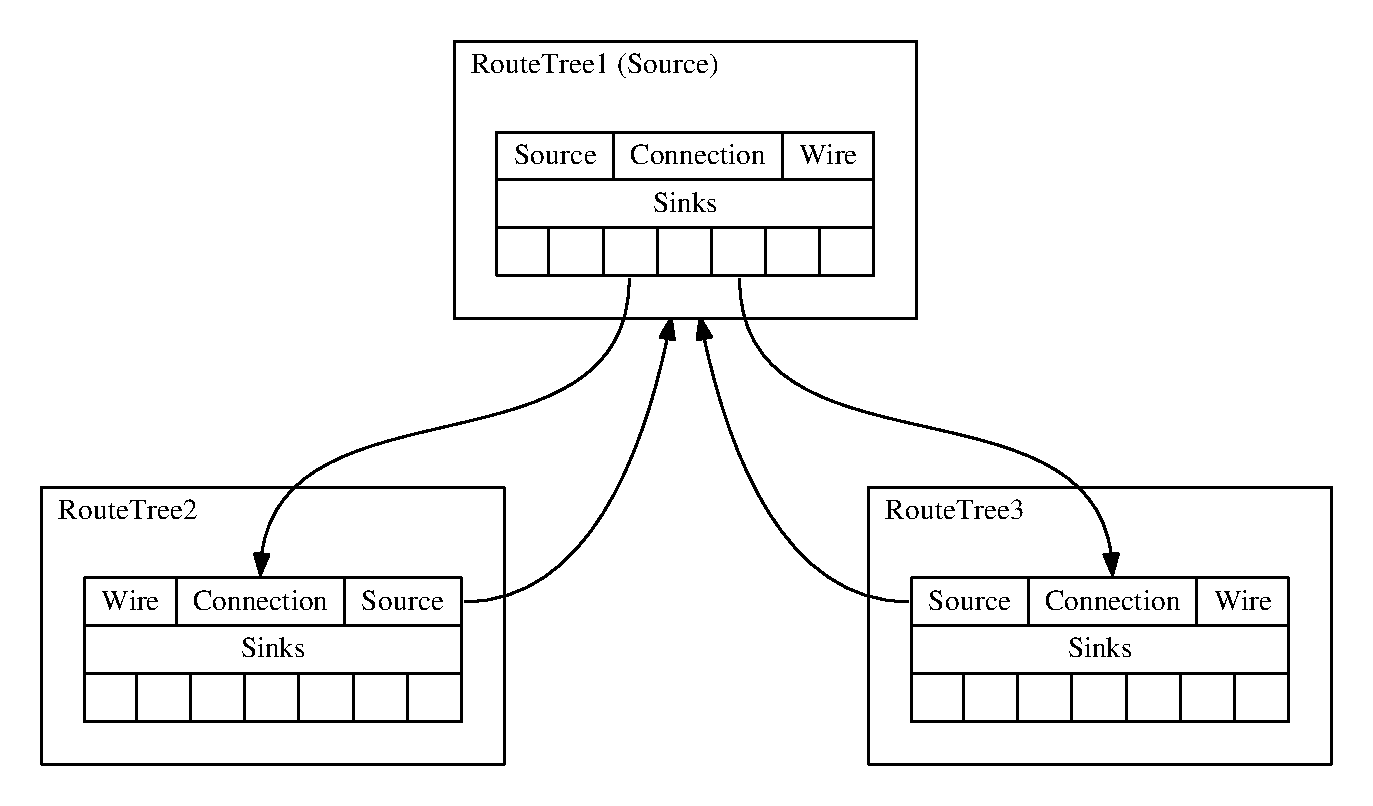
\includegraphics[width=0.8\columnwidth]{routeTreeDS.eps}
\caption{Visual representation of the \cls{RouteTree} data structure.}
\label{fig:routeTreeDS}
\end{figure}

\noindent
As the figure shows, a \cls{RouteTree} is a simple tree data structure. Each
node in the tree represents a physical wire, and is connected to other nodes
(wires). Edges in the tree represent wire connections (i.e. how one wire
connects to another). A \cls{RouteTree} can also be conceptually thought of as
a graph, with a single ``starting'' node and several ``sink'' nodes. A
\cls{RouteTree} node contains the following members:

\begin{itemize}
  \item \pgm{Wire}: The physical \cls{Wire} object that the \cls{RouteTree} node
  represents. This can be either a \cls{TileWire} or \cls{SiteWire}.
  \item \pgm{Source}: A link to the the parent \cls{RouteTree} node 
  \item \pgm{Connection}: The \cls{Connection} taken from the \pgm{parent}
  RouteTree node to reach the \pgm{current} RouteTree node. In other words, it
  is the \cls{WireConnection} object that was taken from the parent wire to reach the current wire.
  \item \pgm{Sinks}: A list of child nodes. There is no limit
  to how many children a \cls{RouteTree} node can have.
  \item \pgm{Cost} (not shown): An optional cost field for routers 
\end{itemize}

\noindent
A complete \cls{RouteTree} specifies how the source of a
\cellnet is physically connected to all of its sinks. \autoref{fig:routeTree}
shows an example of a complete \cls{RouteTree} in RapidSmith. 

\begin{figure}[H]
\centering
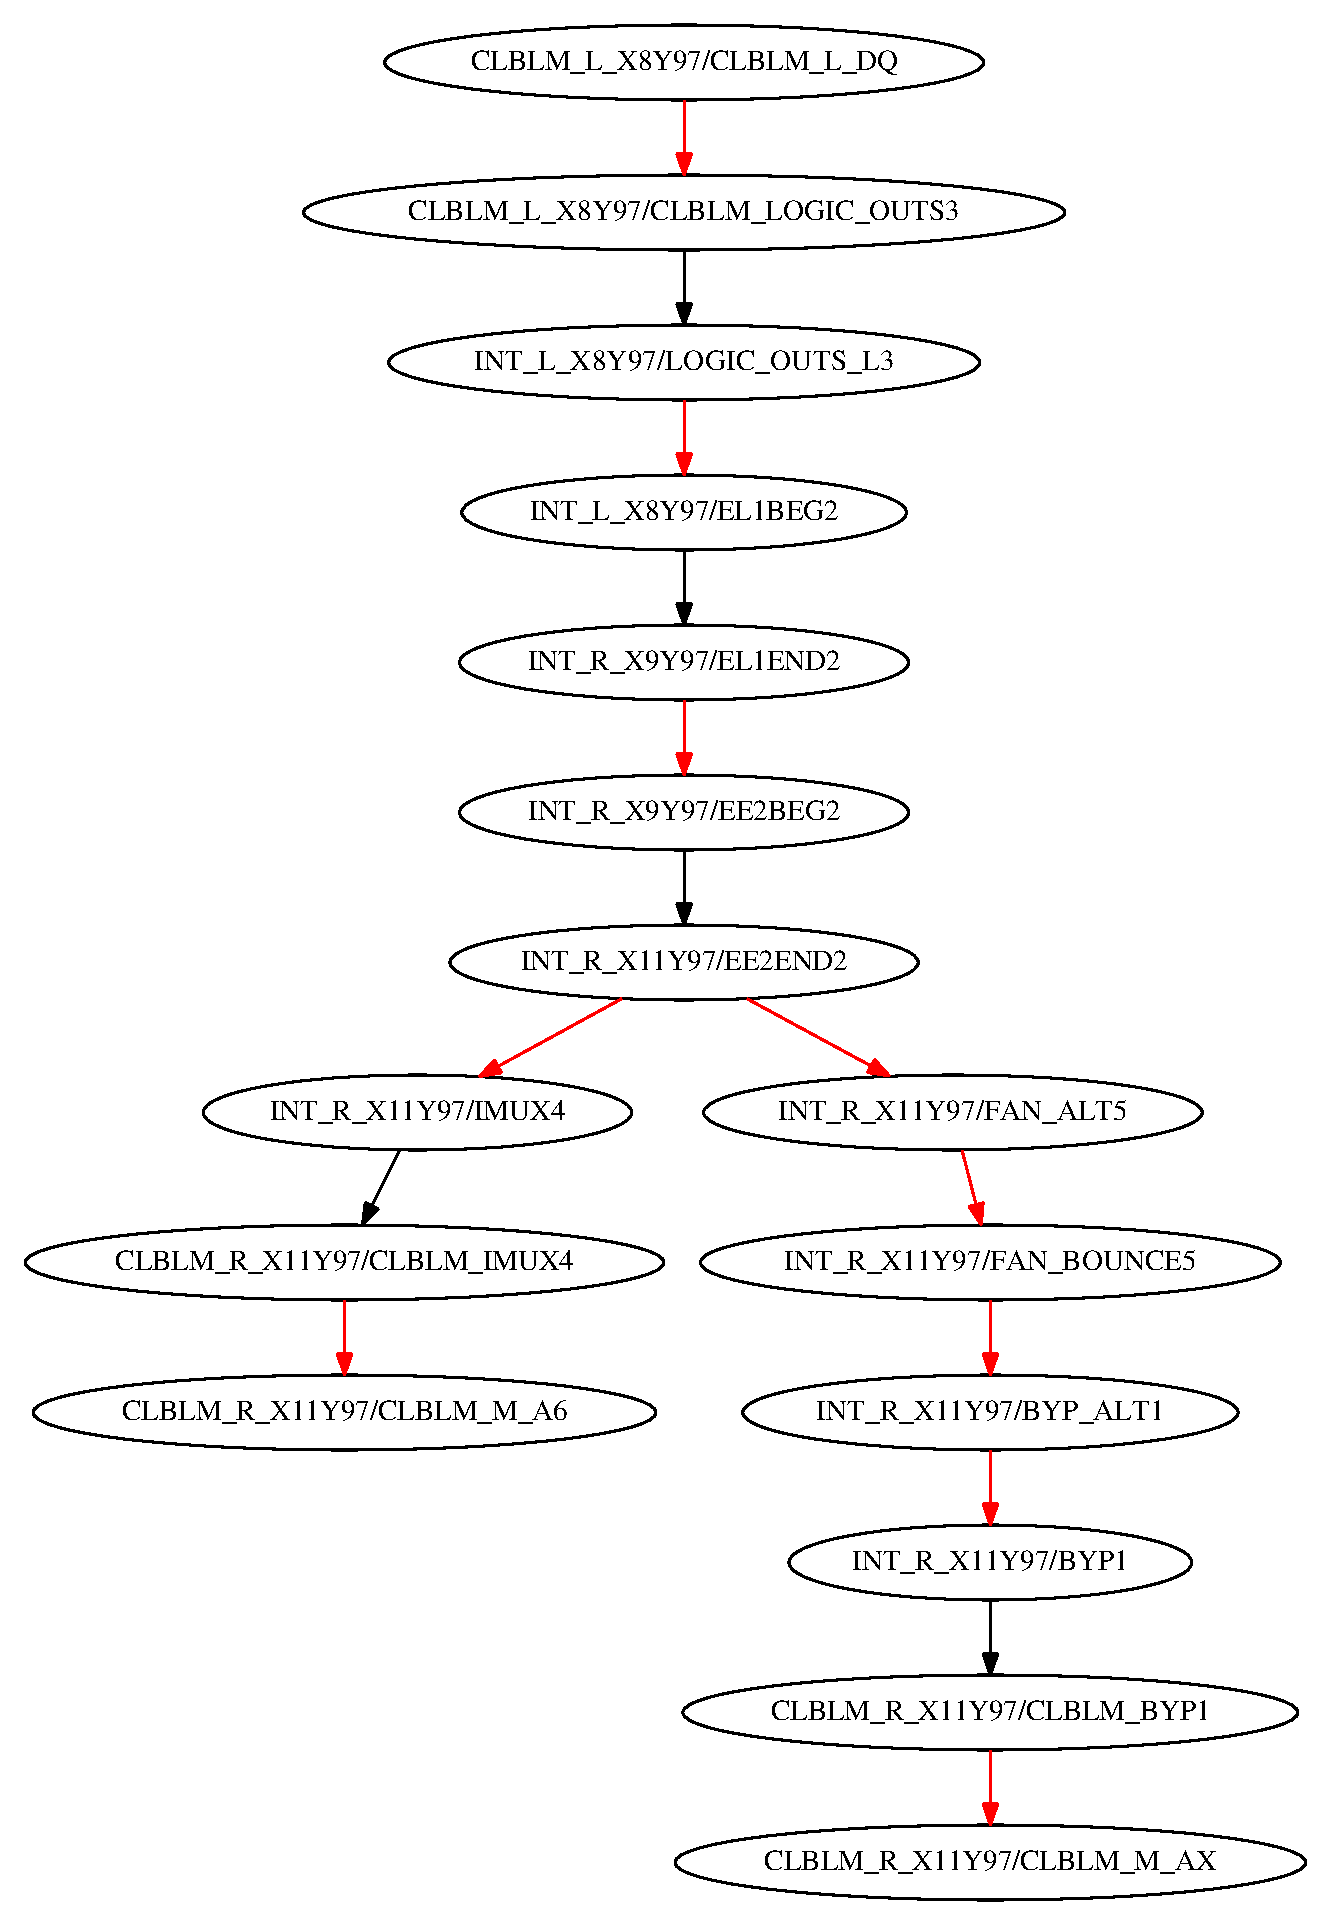
\includegraphics[width=0.65\columnwidth]{routeTree.eps}
\caption{A visual representation of a RapidSmith2 RouteTree. Nodes represent
\cls{Wire}s, red edges represent \cls{PIP} wire connections, and black edges
represent non-PIP wire connections. This specific RouteTree was created from
the \pgm{AStarRouter} example.}
\label{fig:routeTree}
\end{figure}

\noindent
In this case, the \cellnet that is being routed has once source pin, and two
sink pins. The source pin is connected to wire ``CLBLM\_L\_X8Y97/CLBLM\_L\_DQ'',
and the sink pins are connected to the wires ``CLBLM\_R\_X1Y97/CLBLM\-\_M\_A6''
and ``CLBLM\-\_R\_X11Y97/CLBLM\_M\_AX''. Starting from the source, wires are
traversed downward (via wire connections) until the target wires are reached.
\autoref{code:routeTree} demonstrates the basic usage of \cls{RouteTree}s in
RapidSmith. The \pgm{DesignAnalyzer}, \pgm{AStarRouter}, and \pgm{HandRouter}
examples described in \autoref{examples} also demonstrate how to traverse and
build a \cls{RouteTree}.

\begin{lstlisting}[caption=Building a RouteTree,
label=code:routeTree] 
// Find a Wire to start the RouteTree at
Site site = device.getSite("SLICE_X5Y84");
SitePin pin = site.getSitePin("DQ");
Wire startWire = sink.getExternalWire();

// Create the first node in the RouteTree 
Queue<RouteTree> rtQueue = new LinkedList<RouteTree>();
RouteTree start = new RouteTree(startWire);
rtQueue.add(start);

// Build up the RouteTree somehow 
while (!amDone()) {
	RouteTree current = rtQueue.poll();
	Wire wire = route.getWire();

	for (Connection conn : wire.getWireConnections()) {
		// add qualified connections to the RouteTree
		if (isQualified(wire)) {
			RouteTree tmp = current.addConnection(conn);
			rtQueue.add(tmp);
		}
	}
}

\end{lstlisting}

When a design is imported from Vivado, the routing information is parsed and
loaded into \cls{Route\-Tree}s for each \cellnet. On design export, the
\cls{RouteTree} for each \cls{CellNet} is traversed and converted into a Vivado
ROUTE string. A user can use custom data structures to route a design, but it
needs to be \pgm{converted to an equivalent RouteTree data structure} before
exporting the design to Vivado.  

\subsection{Three Part Routing}
In RapidSmith 2, there are three sections to a routed  \cellnet. 

\begin{enumerate}
  \item The portion of the net that starts at the source \belpin, and is routed
  to an output \sitepin. This part of the route exists completely inside of
  \site boundaries.
  \item The portion of the net that starts at the output \sitepin of part (1),
  and is routed to several sink \sitepins. This part of the route is
  called the ``INTERSITE'' route because it connects \sites together. A typical
  router is responsible for routing this section of the net\footnote{VCC and
  GND nets don't follow this pattern. The only difference for VCC and GND is
  that they can have multiple intersite nets.}.
  \item The portion of the net that start at an input \sitepin from part (2),
  and is routed to a sink \belpin. Since there can be several sink pins in a
  \cellnet, this section of the net can have more than one component. This part
  of the route also exists completely inside of \site boundaries. 
\end{enumerate}

\noindent \autoref{fig:threePartRouting} shows an example of the three parts of
a routed \cellnet.

\begin{figure}[H]
\centering
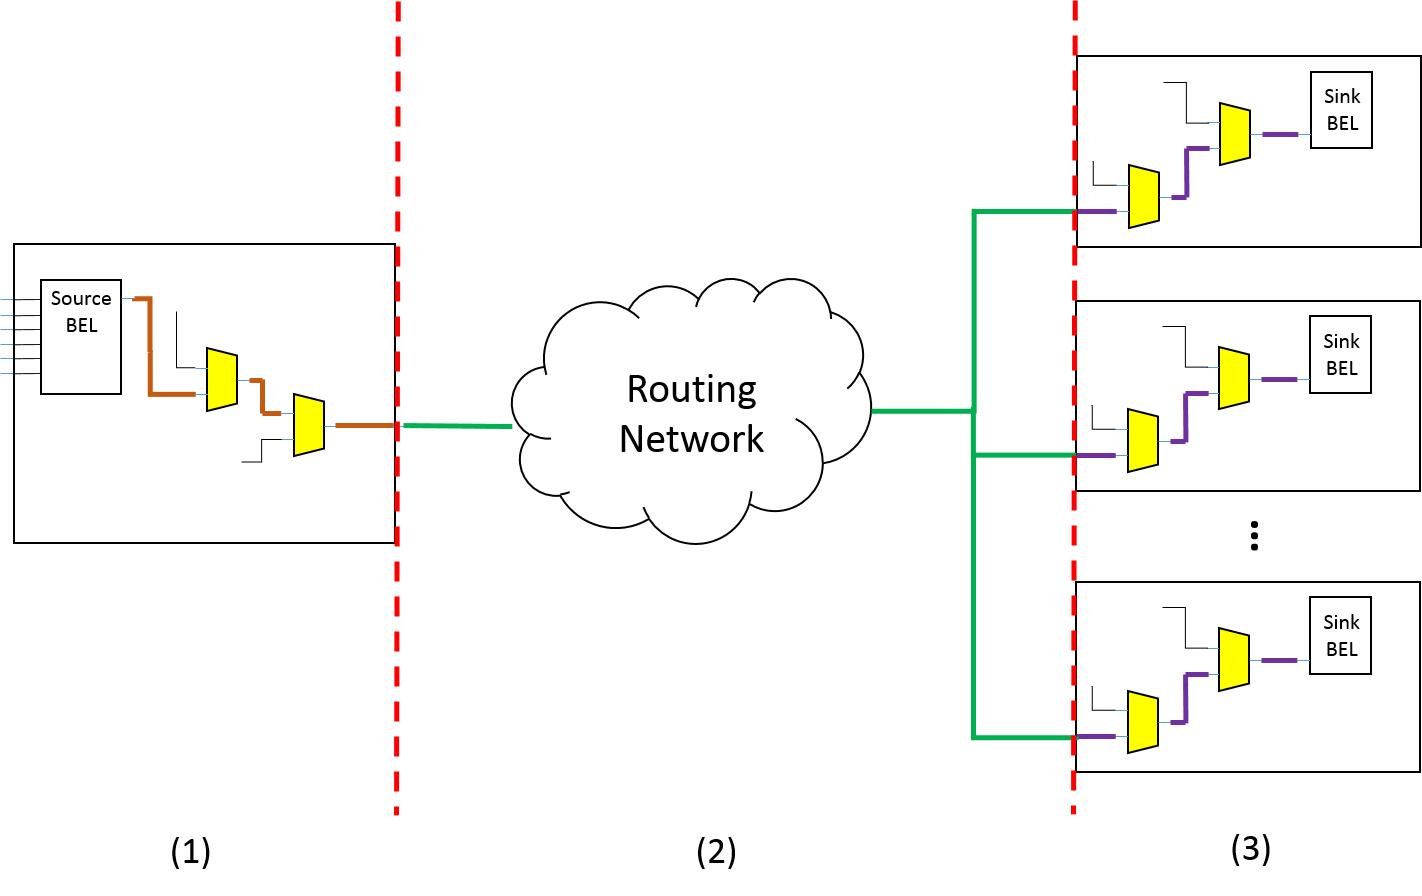
\includegraphics[width=1\columnwidth]{threePartRouting.png}
\caption{The three sections of a RapidSmith route.}
\label{fig:threePartRouting}
\end{figure}

\noindent 
There is a \routeTree object associated with each section of the
three-part routing. A source \routeTree represents the orange wires in the
figure above (part 1). An intersite \routeTree represents the green wires in the
figure above (part 2). A list of sink \routeTrees represents the purple
wires in the figure above (part 3, with a different \routeTree object for each
\site). It is important to note that INTRASITE nets only have a source
\routeTree because they are completely contained within a \site.
\autoref{code:threePartRouting} demonstrates how to utilize three part routing
in RapidSmith. When a design is imported into RapidSmith, the routing sections
of each \cellnet are created automatically.

\begin{lstlisting}[caption=Three-part routing in RapidSmith,
label=code:threePartRouting]
// Get a handle to a routed net in the design 
CellNet net = design.getNet("myNet");

// Handling the source RouteTree
RouteTree source = net.getSourceRouteTree();
net.setSourceRouteTree(createSourceRoute());

// Handling the intersite RouteTree
RouteTree intersite = net.getIntersiteRouteTree();
net.addIntersiteRouteTree(createIntersiteRoute());

// Iterate over a list of sink RouteTrees
for (RouteTree rt : net.getSinkSitePinRouteTrees()) {
	// do something with the RouteTree
}

// Or, get a RouteTree based on a SitePin
for(SitePin sitePin : net.getSitePins()) {
	if (sitePin.isInput()) {
		RouteTree sinkTree = net.getSinkTree(sitePin);
		// do something with the RouteTree
	}
}

// Add a new sink RouteTree that starts at a SitePin

net.addSinkRouteTree(sitePin, createSinkRouteTree(sp));
\end{lstlisting}

\subsection{Routing in Vivado}
The reason a three-part routing distinction is necessary in RapidSmith, is due
to how routing is represented in Vivado. Inside \site boundaries, a route is
represented using \site \pips. A string of enabled \pips determines what pins
are connected together within the \site. Between \site boundaries, a route is
instead represented using wires. The wires are formatted into a Vivado ROUTE
string, which uniquely specifies the intersite route for a net. The three-part
routing representation makes this distinction explicit to the users of
RapidSmith (it also makes import/export easier). When a design is exported from
Vivado, the intrasite portions of a net are exported as \site \pips, and the
intersite portion of the net is exported as wires.

\begin{lstlisting}[numbers=none, keywordstyle=, stringstyle=]
% An example of a string of used site pips in Vivado
{IUSED:0 IBUFDISABLE_SEL:GND INTERMDISABLE_SEL:GND}

% An example of a Vivado ROUTE string
 { CLBLL_LL_AQ CLBLL_LOGIC_OUTS4  { NW6BEG0 NE2BEG0 WR1BEG1 IMUX_L34
IOI_OLOGIC0_D1 LIOI_OLOGIC0_OQ LIOI_O0 }  IMUX_L1 CLBLL_LL_A3 }  
\end{lstlisting}

\subsection{IntrasiteRouting}
On design import, the \site \pip information extracted from Vivado is stored
into RapidSmith data structures, and used to resconstruct the three-part
routing view. This gives the user two options when dealing with intrasite
routing in RapidSmith: (1) use the three-part routing data structures, or (2)
use the set of enabled \site \pips that exist in each \site. It is up to user
preference for which representation to use when writing a CAD tool, but in
order to export a design back into Vivado the three-part routing data
structures need to be converted to \site \pips and assigned to their
corresponding \site. \autoref{code:sitePips} demonstrates how this is
currently done. This step needs to be taken \pgm{only when you have modified the
intrasite routing} for a \site. We are working on improving the API for \site
\pips, and creating a way to automate conversion from three-part routing to
\site \pip information.

\begin{lstlisting}[caption=Configuring Site Pips,
label=code:sitePips]
// Get a handle to a Design and a Site
CellDesign design = tcp.getDesign();
Device device = tcp.getDevice();
Site site = device.getSite("SLICE_X5Y84");

// Get a list of used site wires somehow (this is up to you)
Set<Wire> usedSiteWires = getUsedWires(site);

// Convert the list of wires to their integer enumeration
Set<Integer> usedPipWires = usedSiteWires.stream()
										 .map(w -> w.getWireEnum())
										 .collect(Collectors.toSet());

// Set the used site pips with the design class
design.setUsedSitePipsAtSite(site, usedPipWires);

\end{lstlisting}

\pagebreak
\section{Importing/Exporting Designs Between Vivado and RS2} \label{sec:import}
Importing and exporting designs between Vivado and RS2 is fairly
straightforward. It is done using Tincr Checkpoint (TCP) files, which contain a
variety of information about a digital design. This section describes in detail
the following: 

\begin{itemize}
  \item The contents of TCP files
  \item The small differences between TCP files for design import and export
  \item How to load a TCP into RS2, and how to export a RS2 design to a TCP
  \item Some additional information that is imported with a TCP 
\end{itemize}

\subsection{RapidSmith Checkpoints}
RapidSmith checkpoints (RSCP) are Tincr checkpoints generated in Vivado from the
command \texttt{::tincr::write\-\_rscp}. These checkpoints are capable of
representing a Vivado design at any stage of implementation (post-synthesis,
post-place, and post-route), and can be parsed and imported into RapidSmith. As
we will see in \autoref{sec:tcp} below, the format of these checkpoints differ
slightly than those of regular TCPs. This is because a great deal of additional
information needs to be added to RapidSmith checkpoints in order to import a
complete representation of a Vivado design. The remainder of this subsection
describes each of the file types within a RapidSmith checkpoint, and what they
represent.

\subsubsection{design.info}
The \textit{design.info} file within a RSCP is used to include any useful
information about a design. Currently, it only stores the part name that the
design is implemented on. This file is reserved to add more additional
information in the future.

\subsubsection{netlist.edf}
The \textit{netlist.edf} file within a RSCP is an EDIF netlist representing the
logical portion of a design. It details all of the \cells, \nets,
and \ports within a design, and is generated from Vivado using the Tcl
command \texttt{write\_edif}. A RapidSmith \celldesign is created by parsing the
EDIF file, and converting it into the appropriate RS2 data structures described
in \autoref{sec:designDS}. Below is an example of a RSCP EDIF file.

\begin{lstlisting}[numbers=none, keywordstyle=, stringstyle=]
  (Library work
    (edifLevel 0)
    (technology (numberDefinition ))
   (cell add (celltype GENERIC)
     (view add (viewtype NETLIST)
       (interface 
        (port a (direction INPUT))
        (port b (direction INPUT))
        (port cin (direction INPUT))
        (port cout (direction OUTPUT))
        (port s (direction OUTPUT))
       )
       (contents
         (instance GND (viewref netlist (cellref GND (libraryref hdi_primitives))))
         (instance VCC (viewref netlist (cellref VCC (libraryref hdi_primitives))))
         (instance a_IBUF_inst (viewref netlist (cellref IBUF (libraryref hdi_primitives))))
         (instance b_IBUF_inst (viewref netlist (cellref IBUF (libraryref hdi_primitives))))
         (instance cin_IBUF_inst (viewref netlist (cellref IBUF (libraryref hdi_primitives))))
         (instance cout_OBUF_inst (viewref netlist (cellref OBUF (libraryref hdi_primitives))))
         (instance cout_OBUF_inst_i_1 (viewref netlist (cellref LUT3 (libraryref hdi_primitives)))
           (property INIT (string "8'hE8"))
         )
\end{lstlisting}

\subsubsection{placement.rsc}
The \textit{placement.rsc} file within a RSCP stores all of the placement
information of a Vivado design. This includes which package pin every \port is
mapped to, which \bel each \cell is placed on, and the logical-to-physical pin
mappings for each \cellpin. If a design has not yet been placed, this file
will be empty. Below is an example of a RSCP placement file.

\begin{lstlisting}[numbers=none]
LOC a_IBUF_inst R10 IOB33 INBUF_EN LIOB33_SING_X0Y50
PINMAP a_IBUF_inst O:OUT I:PAD 
LOC b_IBUF_inst T10 IOB33 INBUF_EN LIOB33_X0Y51
PINMAP b_IBUF_inst O:OUT I:PAD 
LOC cin_IBUF_inst T9 IOB33 INBUF_EN LIOB33_X0Y51
PINMAP cin_IBUF_inst O:OUT I:PAD 
LOC cout_OBUF_inst U13 IOB33 OUTBUF LIOB33_X0Y53
PINMAP cout_OBUF_inst O:OUT I:IN 
LOC cout_OBUF_inst_i_1 SLICE_X0Y51 SLICEL A6LUT CLBLL_L_X2Y51
PINMAP cout_OBUF_inst_i_1 O:O6 I0:A4 I1:A5 I2:A6 
LOC s_OBUF_inst T13 IOB33 OUTBUF LIOB33_X0Y53
PINMAP s_OBUF_inst O:OUT I:IN T:TRI 
PACKAGE_PIN R10 a
PACKAGE_PIN T10 b
PACKAGE_PIN T9 cin
PACKAGE_PIN U13 cout
PACKAGE_PIN T13 s
\end{lstlisting}

\subsubsection{routing.rsc}
The \textit{routing.rsc} file within a RSCP stores all of the routing
information of a Vivado design. This includes: 

\begin{itemize}
  \item The used \cls{Site} \cls{PIPs} within each \cls{Site} (which
  specifies the internal routing)
  \item A list of LUT \bels that are acting as static sources (see
  \autoref{sec:additionalInfo} for more details)
  \item A list of LUT \bels that are being used as routethroughs (see
  \autoref{sec:additionalInfo} for more details) 
  \item The name of each INTRASITE net
  \item The name, connecting \cls{SitePin}s, and used \cls{TileWire}s
  of each INTERSITE net.
  \item Special routing information for the VCC and GND nets.
\end{itemize}

\noindent
If Vivado has not yet been routed, this file will be mostly empty. Below is
an example of the contents within a RSCP routing file.

\begin{lstlisting}[numbers=none]
SITE_PIPS SLICE_X9Y80 SRUSEDMUX:0 CEUSEDMUX:IN COUTUSED:0 CLKINV:CLK DCY0:DX ...
SITE_PIPS SLICE_X13Y80 PRECYINIT:AX SRUSEDMUX:0 CEUSEDMUX:IN COUTUSED:0 ...
SITE_PIPS SLICE_X15Y80 SRUSEDMUX:0 CEUSEDMUX:IN COUTUSED:0 CLKINV:CLK DCY0:DX ...
SITE_PIPS M17 OUSED:0 

... 

STATIC_SOURCES SLICE_X2Y106/D6LUT/O6 SLICE_X2Y106/C6LUT/O6 SLICE_X4Y106/D6LUT/O6 ...
LUT_RTS SLICE_X5Y101/B6LUT/A6/O6 SLICE_X2Y100/A5LUT/A4/O5 SLICE_X5Y100/C6LUT/A6/O6 ...

...

INTRASITE AddSub[10]
INTERSITE AngStep1[0] SLICE_X2Y82/AX SLICE_X2Y87/AQ SLICE_X2Y84/A1
ROUTE AngStep1[0] CLBLM_R_X3Y87/CLBLM_M_AQ CLBLM_R_X3Y87/CLBLM_LOGIC_OUTS4 ...

...

VCC INT_L_X2Y107/VCC_WIRE INT_L_X2Y107/VCC_WIRE INT_L_X2Y107/VCC_WIRE ...
START_WIRES INT_L_X2Y107/VCC_WIRE INT_L_X2Y106/VCC_WIRE INT_R_X3Y106/VCC_WIRE ...
GND INT_R_X3Y106/GND_WIRE INT_R_X3Y106/GND_WIRE INT_R_X3Y106/GFAN1 ...
START_WIRES INT_R_X3Y106/GND_WIRE INT_L_X4Y106/GND_WIRE INT_R_X3Y105/GND_WIRE ...
\end{lstlisting}

\subsubsection{contraints.rsc}
The \textit{contraints.rsc} file within a RSCP stores all XDC constraints on a
Vivado design. XDC constraints are similar to UCF files for ISE designs. They
can be used to set the clock frequency, constrain a top-level port to a specific
package pin on the device, and set other physical implementation details. An
example of a RSCP constraints file can be seen below.

\begin{lstlisting}[numbers=none]
create_clock -period 5.000 -name sysClk -waveform {0.000 2.500}
set_property IOSTANDARD LVCMOS18 [get_ports clk]
set_property IOSTANDARD LVCMOS18 [get_ports ena]
set_property PACKAGE_PIN E15 [get_ports {Yin[12]}]
set_property PACKAGE_PIN H17 [get_ports {Xin[14]}]
set_property PACKAGE_PIN D18 [get_ports {Xin[7]}]
\end{lstlisting}

\noindent
As can be seen, a Vivado constraints file is essentially a list of Tcl commands
to execute before generating a bitstream. When importing a RSCP into RapidSmith,
each constraint is parsed into a \cls{XdcConstraint} object and stored in the
top-level \celldesign. Each \cls{XdcConstraint} has two fields, a String
command and a String representing all command arguments. \autoref{code:xdc}
demonstrates how to manipulate XDC constraints in RapidSmith. Future RS2 plans
include creating a more intelligent way of handling XDC constraints. 

\begin{lstlisting} [caption=How to manipulate XDC constraints in RS2,
label=code:xdc] 
// Getting a list of all constraints in the current design
List<XdcConstraint> xdcConstraints = design.getVivadoConstraints();

// Look for all of the "create_clock" constraints in the design
List<XdcConstraint> crtClks = xdcConstraints.stream()
                              .filter(xdc -> xdc.getCommandName().equals("create_clock")) 
                              .collect(Collectors.toList());

// Add a new XDC constraint to the design
XdcConstraint xdc = new XdcConstraint("set_property", "IOSTANDARD LVCMOS18 [get_ports clk]") 
design.addVivadoConstraint(xdc);
\end{lstlisting}

\subsection{Tincr Checkpoints} \label{sec:tcp}
Tincr checkpoints are very similar to RapidSmith checkpoints, but they can be
used to import designs back into Vivado after they have been modified in
RapidSmith. The main different between TCPs and RSCPs, is that the
\textit{placement.rsc}, \textit{routing.rsc}, and \textit{constraints.rsc} files
turn into \textit{placement.xdc}, \textit{routing.xdc}, and \textit{constraints.xdc}
respectively. Vivado is able to parse the XDC files and apply physical
information to the design. On design export, RapidSmith produces
a TCP that is compatible with Vivado. The file formats of the three XDC files
will not be included in this documentation. If you are interested in their
format, the best way to learn is to consult the Vivado user guide and generate a
TCP from RapidSmith and view the individual files.

\subsection{Additional Information} \label{sec:additionalInfo}
The reason RSCP and TCP checkpoints are distinguished, is that there are
several design implementation aspects in Vivado that aren't explictly
represented. In order to accurately represent a design in RapidSmith, they
must be included somehow. This section describes the parts of the design that
aren't explicitly represented in Vivado, and how RapidSmith handles them.
\autoref{sec:importExportTcp} describes how to get a handle to the additional
information after a checkpoint has been imported.

\subsubsection{LUT Routethroughs}
Besides their use in implementing logic equations, LUT BELs can also act as
signal routethroughs. In Vivado, a LUT is marked as a  routethrough when its
configuration equation (CONFIG.EQN) maps the value of a single input pin
directly to the output pin. These LUTs are not explicitly represented in the
logical netlist because there is no cell placed on the corresponding BEL. 
\autoref{fig:routethroughs} shows two examples of LUTs in Vivado that are
configured as routethroughs.

\begin{figure}[h]
  \centering
  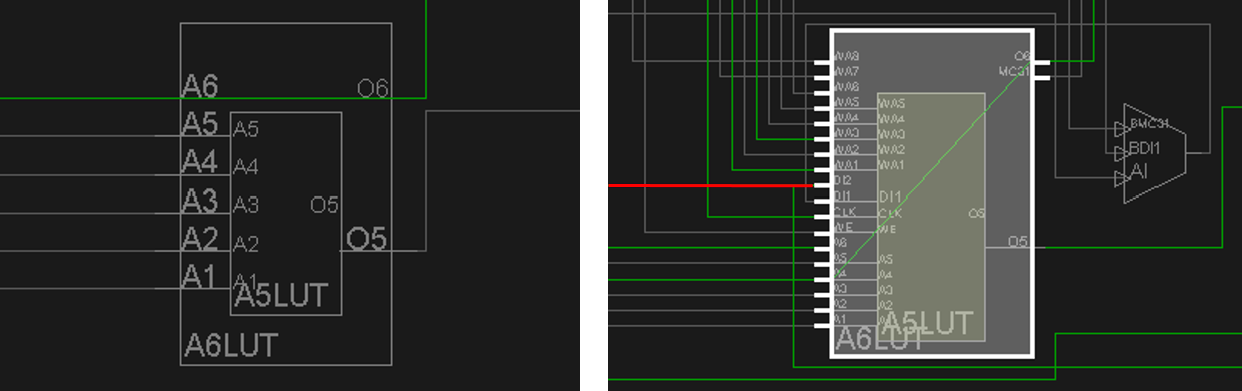
\includegraphics[width=1\columnwidth]{routethroughs}
  \caption{Two examples of LUTs being used as
  routethroughs in the Vivado GUI. The RT on the left uses the A6 input pin,
  while the RT on the right uses the A4 input pin. The net highlighted in red
  represents VCC.}
  \label{fig:routethroughs}
\end{figure}

\noindent
When a design is exported from Vivado, all LUTs that are acting as routethroughs
are included in the \textit{routing.rsc} file of a RSCP. When the file is
parsed, each routethrough is stored in a \cls{BelRoutethrough} object which
contains the physical \bel, the input \belpin, and the output \belpin that
uniquely describes the routethrough. It is important to note that if a \bel is
being used as a routethrough, no \cell can be placed there. When creating CAD
tools, \cls{BelRoutethrough}s give the user a more complete picture of what
\bels are actually available. 
	
As described in \autoref{otherConns}, there is a \cls{Connection} object in
RapidSmith from every input LUT pin to the LUTs output pin. These \bel
routethrough connections, are actually just \cls{WireConnection}s with the
\texttt{isRoute\-through()} method returning true. In order to use a LUT as a
routethrough in RapidSmith, you simply have to include the corresponding
\cls{WireConnection} within an INTRASITE \cls{RouteTree}. When a design is
exported from RapidSmith, the routethrough \cls{WireConnection}s are
automatically detected and converted to a passthrough LUT \cell. The netlist
is rewired appropriately.

\subsubsection{Static Source LUTs}
LUTs can also act as a static power or ground source. This occurs when the
configuration equation is set to 1 or 0. An example of a LUT that exhibits
this behavior is shown in \autoref{fig:staticSourceLut}. When a design
is exported from Vivado, all LUTs that are acting as static sources are
included in the \textit{routing.rsc} file of a RSCP. As the file is being
parsed, a list of static sources \bels are recorded and stored in a list data
structure. Just like routethroughs, if a \bel is being used as a static source
no \cell should be placed on it.

\begin{figure}[h]
  \centering
  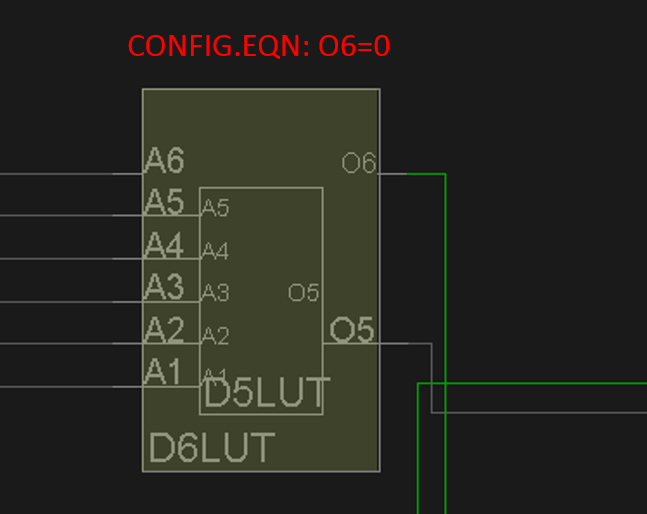
\includegraphics[width=.5\columnwidth]{staticSourceLut.png}
  \caption{A LUT \bel that has been configured as a GND source. Notice that
  there are no input pins being driven.}
  \label{fig:staticSourceLut}
\end{figure}

\subsubsection{Pseudo CellPins}
\cls{PseudoCellPin}s are described in great detail in \autoref{sec:cellPin}.
When a RSCP is loaded, \cls{PseudoCellPin}s are automatically detected,
created, and attached to their corresponding \cells.

\subsection{Importing and Exporting TCPs} \label{sec:importExportTcp}
After a Vivado design has been converted to a TCP using the
\texttt{::tincr::write\_rscp} command, it can be loaded into RapidSmith.
\autoref{code:import} demonstrates the basix syntax of design
import and export.

\begin{lstlisting}[caption=How to import and export TCP files to and from RS2,
label=code:import]
// Loading a Tincr Checkpoint
TincrCheckpoint tcp = VivadoInterface.loadTcp("pathToCheckpoint.tcp");
CellDesign design = tcp.getDesign();
Device device = tcp.getDevice();
CellLibrary libCells = tcp.getLibCells();

// Insert CAD Tool Here

// Exporting the modified design to a Tincr Checkpoint
VivadoInterface.writeTCP("pathToStore.tcp", design, device, libCells);

\end{lstlisting}

\noindent
While a design is being imported into RapidSmith, several useful data structures
are built up. If you want to gain access to those data structures, you can pass
an additional argument into the \texttt{VivadoInterface.loadTCP} method. This
is shown in \autoref{code:import2}.

\begin{lstlisting}[caption=Importing a TCP with additional information,
label=code:import2]
// Loading a Tincr Checkpoint with additional info
TincrCheckpoint tcp = VivadoInterface.loadTcp("PathToCheckpoint.tcp", true);
Collection<BelRoutethrough> belRts = tcp.getRoutethroughObjects();
Collection<Bel> staticSources = tcp.getStaticSourceBels();
Map<BelPin, CellPin> belPinToCellPinMap = tcp.getBelPinToCellPinMap()
\end{lstlisting}

\pagebreak
\section{Example Programs} \label{examples}

A variety of example programs can be found in the
\pkg{edu.byu.edu.rapidSmith.examples} package of the RS2 installation.
They have been heavily commented to provide a means to learn the RS2 API by
example. We believe this approach is better than reading through a block of
text while trying to understand the data structures and what they do.
There is a \fil{README.txt} file in that directory to provide an overview of
each example. The order that they appear in the \fil{README.txt} is also the
suggested learning order for beginners. In addition, the subsections below
describe one or more built-in RS2 programs which you might find useful.

\subsection{Sample Vivado Designs}
To enable new users of RS2 to quickly start running the example
programs, a small set of pre-compiled Vivado designs have been included in the
distribution. They are located in the \dir{exampleVivadoDesigns} directory of
the repository, and consist of 3 designs: 
\begin{itemize}
\item \textbf{add.tcp}: synthesized only
\item \textbf{cordic.tcp}: synthesized and placed
\item \textbf{count16.tcp}: synthesized, placed and routed
\end{itemize} 
There is a sample design to demonstrate each possible tool flow between Vivado
and RS2. Equivalent Vivado checkpoints files (.dcp) are also included in
the same directory as \fil{add.dcp}, \fil{cordic.dcp}, and \fil{count16.dcp}
files. To open these checkpoints in Vivado, you can either (a) double click on
the .dcp file in a file explorer, or (b) use the command
\texttt{open\_checkpoint} when a Vivado terminal is open. It is suggested that
you have the equivalent Vivado designs open when going through the example
programs listed below.

If you want to recompile the designs from scratch, the source code for each
design has also been included in the same directory. The Tcl script called
\pgm{compile.tcl} can be used for this purpose. Simply open Vivado in Tcl
mode, and type the following commands to re-build one of the example designs. 
                
\vspace{-0.15in}  \begin{code}
	Vivado\% cd <path to exampleVivadoDesigns directory>
	Vivado\% compile_hdl_to_checkpoint_files add
	Vivado\% close_project
\end{code}
This will synthesize, place, and route a design and, from that compiled
design, generate the \dir{.tcp} directory and the \fil{.dcp} file. For example
programs that only explore the architecture, opening the device browser in
Vivado can also be helpful.

\subsection{\pgm{DeviceBrowser}}
The DeviceBrowser is a GUI program located in the 
\pkg{edu.byu.ece.rapidSmith.device.browser} package. It lets you browse
parts at the tile level, and is useful for becoming more familiar with FPGA
architecture. As long as a valid device file exists, then the DeviceBrowser can
operate (no design required). A screenshot from the DeviceBrowser can be seen in
\autoref{fig:deviceBrowser}. On the left, the user may choose the desired part
by navigating the tree menu and double-clicking on the desired part name.
This will load the part in the viewer pane on the right (the first available
part is loaded at startup). The status bar in the bottom left displays which
part is currently loaded. Also displayed is the name of the current tile
which the mouse is over, highlighted by a yellow outline in the viewer pane.
The user may navigate inside the viewer pane by using the mouse. By
right-clicking and dragging the cursor, the user may pan. By using the
scroll-wheel on the mouse, the user may zoom. If a scroll-wheel is
unavailable, the user may zoom by clicking inside the viewer pane and pressing
the minus(-) key to zoom out or the equals(=) key to zoom in.

\begin{figure}[htb]
\centering
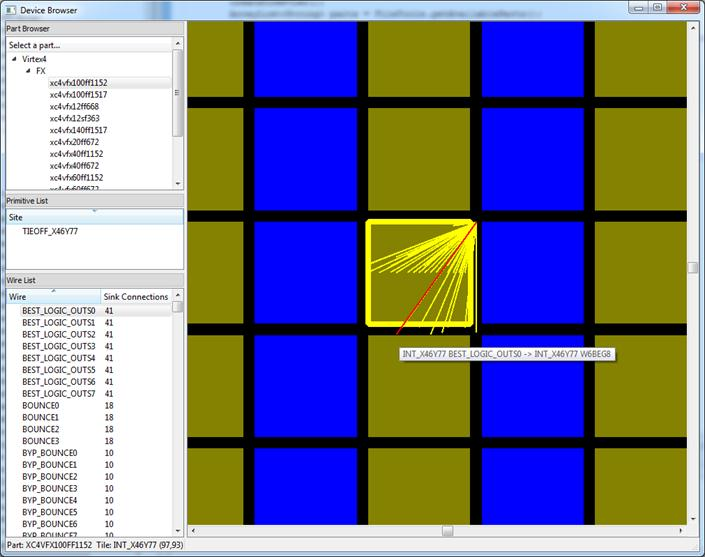
\includegraphics[width=0.8\columnwidth]{deviceBrowser2}
\caption{\pgm{DeviceBrowser} Screen Shot Showing Wire Connections}
\label{fig:deviceBrowser2}
\end{figure}

The device browser also allows the user to follow the various connections found
in the FPGA.  By double clicking a wire in the wire list, the application will
draw the connection on the tile array (as shown in
\autoref{fig:deviceBrowser2}). By hovering the mouse pointer over the
connection, the wire becomes red and a tooltip will appear describing the
connection made by declaring the source tile and wire followed by an arrow and
the destination tile and wire.  By clicking on the wire, the application will
redraw all the connections that can be made from the currently selected wire. 
By repeating this action, the user can follow connections and discover how the
FPGA interconnect is laid out. Thanks to Chris Lavin for originally creating
this application.

\subsection{\pgm{DeviceAnalyzer}}
The DeviceAnalyzer is designed as a simple getting started program and
demonstrates how to use some of the Device data structures in RS2. This
includes how to query for and print tiles in a device, how to use wires and
wire connections, and other useful device functions.

\subsection{\pgm{ImportExportExample}} \label{sec:importExportExample}
The ImportExportExample demonstrates how to load a Tincr checkpoint into
RapidSmith, and how to export a RapidSmith netlist back into a Tincr
checkpoint. This is a very important step in passing digital designs back
and forth between Vivado and RapidSmith.

\subsection{\pgm{DesignAnalyzer}}
The DesignAnalyzer loads a Tincr checkpoint into RapidSmith, walks
the design data structures, and prints what it finds as it goes in a
readable format. As such, it provides a nice example of a number of things which would
be useful for getting started with RS2 including:
\begin{itemize}
  \item How to enumerate the Cells in a design, determine and print their 
  placement information, and determine and print their properties.
  \item How to enumerate the logical nets in a design and print out their source
  and sink pins. 
  \item How to traverse and print out the physical route for a logical net (if
  it is routed)  
\end{itemize}

\subsection{CreateDesignExample} \label{sec:createDesignExample}
The CreateDesignExample program builds a RapidSmith netlist from scratch (using
\cells and \cellnets) and then places the design. While this is certainly not
recommended for substantial designs, it does demonstrate how to do the
following useful tasks in RapidSmith:

\begin{itemize}
  \item Create new \cells and add them to an existing netlist
  \item Create new \cellnets, and connect them to \cls{CellPin}s
  \item Modify the properties on \cells
  \item Place \cells onto a \bels
  \item Find compatible \bel placement for a given \cell
\end{itemize}

\subsection{Other Test Programs}
The programs introduced in this section are designed for beginners of RS2. Once
you start becoming more comfortable with RapidSmith and its data structures,
there are several other more advanced examples. These examples include the
\pgm{HandRouter}, \pgm{AStarRouter}, and \pgm{SimulatedAnnealingPlacer}
programs. See the README.txt file for more information about each of these
examples.

\pagebreak
\section{Bitstreams in RS2}

In the original RapidSmith, bitstreams can be parsed, manipulated, and exported
for Virtex 4, Virtex 5 and Virtex 6 Xilinx FPGA families.  Because of the
proprietary nature of Xilinx bitstreams, RapidSmith provided only documented
functionality when working with bitstreams (and was limited mainly to
manipulation at the frame level including helping to assemble sequences of
configuration commands which are interpreted by the FPGA configuration
controller circuitry).  While this has proven valuable to many researchers, it
does not provide the ability to create your own bitstream from scratch because
it does not provide the specific meaning of each bit in a bitstream.

If you desire to use RapidSmith's bitstream manipulation features, you should
download and work with RapidSmith instead of RS2 (the RapidSmith bitstream
packages have been removed from RS2).  If you do so, note that RapidSmith's
bitstream packages have not been tested beyond Virtex 6.  The authors would be
interested in upgrading RapidSmith's bitstream functionality to device families
beyond Virtex 6 if users create it and are willing to contribute it to us for
inclusion.

\pagebreak
\section{Installing New Device Files}
By default, RapidSmith includes an Artix7 {\em xc7a100tcsg324} part.
This part has been well tested, and is a good place to start if you are
learning how to use RapidSmith. However, different devices can also be created.
This section describes the necessary steps to create new device files.

\pgm{TODO section}.

\pagebreak
\section{Legal and Dependencies}
RS2 is released under GPL version 3 with the following license: 

\begin{verbatim}
BYU RapidSmith Tools

Copyright (c) 2010-2016 Brigham Young University
   
BYU RapidSmith Tools is free software: you may redistribute it
and/or modify it under the terms of the GNU General Public License
as published by the Free Software Foundation, either version 2 of
the License, or (at your option) any later version.
   
BYU RapidSmith Tools is distributed in the hope that it will be
useful, but WITHOUT ANY WARRANTY; without even the implied warranty
of MERCHANTABILITY or FITNESS FOR A PARTICULAR PURPOSE. See the GNU
General Public License for more details.
   
A copy of the GNU General Public License is included with the BYU
RapidSmith Tools. It can be found at doc/gpl2.txt. You may also get
a copy of the license at http://www.gnu.org/licenses/.
\end{verbatim}

\pagebreak
\section{Included Dependency Projects}
RS2 includes the Caucho Technology Hessian implementation which is distributed
under the Apache License. A copy of this license is included in the doc
directory in the file APACHE2-LICENSE.txt. This license is also available for
download at:

\noindent
\hyperref[http://www.apache.org/licenses/LICENSE-2.0]{\color{blue}http://www.apache.org/licenses/LICENSE-2.0}

\bigbreak \noindent
The source for the Caucho Technology Hessian implementation is available at:

\noindent
\hyperref[http://hessian.caucho.com]{\color{blue}http://hessian.caucho.com}

\bigbreak \noindent
RS2 also includes the Qt Jambi project jars for Windows, Linux and Mac OS X.  Qt
Jambi is distributed under the LGPL GPL3 license and copies of this license and
exception are also available in the /doc directory in files LICENSE.GPL3.TXT and
LICENSE.LGPL.TXT respectively. These licenses can also be downloaded at:

\noindent
\hyperref[http://www.gnu.org/licenses/licenses.html]{\color{blue}http://www.gnu.org/licenses/licenses.html}

\bigbreak \noindent
Source for the Qt Jambi project is available at:

\noindent
\hyperref[http://qtjambi.org/downloads]{\color{blue}http://qtjambi.org/downloads}, and

\noindent
\hyperref[https://sourceforge.net/projects/qtjambi/files/]{\color{blue}https://sourceforge.net/projects/qtjambi/files/}

\bigbreak \noindent
RS2 also includes the JOpt Simple option parser which is released under
the open source MIT License which can be found in this directory in the file
MIT\_LICENSE.TXT.  A copy of this license can also be found at:

\noindent
\hyperref[http://www.opensource.org/licenses/mit-license.php]{\color{blue}http://www.opensource.org/licenses/mit-license.php}

\bigbreak \noindent   
A copy of the source for JOpt Simple can also be downloaded at:

\noindent
\hyperref[http://jopt-simple.sourceforge.net/download.html]{\color{blue}http://jopt-simple.sourceforge.net/download.html}

\bigbreak \noindent
RS2 also includes the JDOM jars.  JDOM is available under an Apache-style open
source license, with the acknowledgment clause removed. This license is among
the least restrictive license available, enabling developers to use JDOM in
creating new products without requiring them to release their own products as
open source. This is the license model used by the Apache Project, which created
the Apache server. The license is available at the top of every source file and
in LICENSE.txt in the root of the JDOM distribution.              

\bigbreak \noindent
The user is responsible for providing copies of these licenses and making
available the source code of these projects when redistributing these jars.

\section{Appendix}
TBD

\end{document}


%%% Local Variables: 
%%% mode: latex
%%% TeX-master: "main"
%%% End: 
